\graphicspath{{Chapter2/Figs/}}

\section{Multi-Omics Factor Analysis: a framework for unsupervised integration of multi-omics data sets}
% In the first section of this chapter, we will describe XXX

The work described in this chapter results from a collaboration with the Multi-omics and statistical computing group lead by Wolfgang Huber at the EMBL (Heidelberg, Germany). It has been peer-reviewed and published in \cite{Argelaguet2018}.\\

The method was conceived by Florian Buettner, Oliver Stegle and me. I performed most of the mathematical derivations and implementation, but with significant contributions from Damien Arnol and Britta Velten. The single-cell application was led by me whereas the CLL data application was led by Britta Velten, but with joint contributions in either cases. Florian Buettner, Wolfgang Huber and Oliver Stegle supervised the project.\\
The article was jointly written by Britta Velten, Florian Buettner, Wolfgang Huber, Oliver Stegle and me.


\subsection{Model description} \label{mofa:model_description}
MOFA is a multi-view generalisation of traditional Factor Analysis to $M$ input matrices (or views) $\bfY^m \in \R^{N \times D_m}$ based on the framework of Group Factor Analysis (discussed in Section X).\\
The input data consists on $M$ views with non-overlapping features that often represent different assays. However, there is flexibility in the definition of views and they can be tailored to address different hypothesis.\\
%For example, if one has DNA methylation data, one could define as a single view the matrix with all genome-wide measurements, but one could also split this matrix into different views, either by chromosome or by genomic context (i.e. promoters, enhancers, etc.).\\
Formally, the input data is factorised as:
\begin{equation}
	\mathbf{Y}^m = \mathbf{Z}\mathbf{W}^{mT} + \bepsilon^m
\end{equation}
where $\bfZ \in \R^{N \times K}$ is a matrix that contains the factor values and $\bfW^m \in \R^{D_m \times K}$ are $M$ matrices that contain the loadings that relate the high-dimensional space to the low-dimensional latent representation. Finally, $\bepsilon^m \in \R^{D_m}$ captures the residuals, or the noise, which is assumed to be normally distributed and heteroskedastic:
\begin{equation}
	p(\epsilon^m_d) = \Ndist{\epsilon^m_d}{0,1/\tau_d^m}
\end{equation}
Non-gaussian noise models can also be defined (see \Cref{section:mofa_ngaussian}). Unless otherwise stated, we will always assume Gaussian noise.\\
Altogether, this results in the following likelihood:
\begin{equation}
	p(\bfY|\bfW,\bfZ,\bTau) = \prod_{m=1}^{M} \prod_{d=1}^{D_m} \prod_{n=1}^{N} \Ndist{y_{nd}^m}{\bfz_{n}^T\bfw_{d}^{m},1/\tau_d^m}
	% p(y_{nd}^m) = \Ndist{y_{nd}^m}{\bfz_{n,:}\bfw_{d,:}^{mT},1/\tau_d^m},
\end{equation}

\subsubsection{Interpretation of the factors}
Each factor ordinates cells along a one-dimensional axis centered at zero. Samples with different signs indicate opposite phenotypes, with higher absolute value indicating a stronger effect. For example, if the $k$-th factor captures the variability associated with cell cycle, we could expect cells in the Mitosis state to be at one end of the factor (irrespective of the sign, only the relative positioning being of importance). In contrast, cells in G1 phase are expected to be at the other end of the factor. Cells with intermediate phenotype, or with no clear phenotype (i.e. no cell cycle genes profiled), are expected to be located around zero, as specified by the prior distribution.

\subsubsection{Interpretation of the loadings}
The loadings provide a score for each gene on each factor, and are interpreted in a similar way as the factors. Genes with no association with the factor are expected to have values close to zero, as specified by the prior. In contrast, genes with strong association with the factor are expected to have large absolute values. The sign of the loading indicates the direction of the effect: a positive loading indicates that the feature is more active in the cells with positive factor values, and viceversa. \\
Following the cell cycle example from above, we expect genes that are upregulated in the M phase to have large positive loadings, whereas genes that are downregulated in the M phase (or, equivalently, upregulated in the G1 phase) are expected to have large negative loadings.\\

% The following figure shows a real-case example of a Factor capturing the cell cycle effect, with the corresponding loadings:

% \begin{figure}[H]
% 	\begin{center}
% 		\includegraphics[width=1.0\textwidth]{figures/cell_cycle}
% 		\caption{Example of a factor (Factor 2) that captures the cell cycle phenotype. Left shows a scatterplot of Factor 1 and Factor 2, where each dot is a single cell. The cells are colored by the infered lineage and they are shaped by the infered cell cycle phase. Right shows the RNA expression loadings for Factor 5. Each dot represents a gene.  }
% 		\label{fig:cell_cycle}
% 	\end{center}
% \end{figure}


\subsubsection{Interpretation of the noise}
The use of a probabilistic framework allows the model to explicitly disentangle the signal (i.e. the explained variance) from the noise (i.e. unexplained variance). Large values of $\tau_d^m$ indicate high certainity on the observations for the feature $d$ in view $m$, as predicted by the latent variables. In contrast, small values of $\tau_d^m$ are indicative of low predictive power by the latent variables.

\subsubsection{Missing values} \label{section:mofa_missing_values}
The probabilistic formalism naturally accounts for incomplete data matrices, as missing observations do not intervene in the likelihood.\\
In practice, we implement this using memory-efficient binary masks $\mathcal{O}^m \in \mathbb{R}^{N\times D_m}$ for each view $m$, such that $\mathcal{O}_{n,d} = 1$ when feature $d$ is observed for sample $n$, 0 otherwise. 

\subsubsection{Prior distributions for the factors and the loadings}  \label{section:mofa_loadings}
The key determinant of the model is the regularization used on the prior distributions of the factors and the weights.\\
For the factors, we define an isotropic Gaussian prior:
\begin{equation}
	p(z_{nk}) = \Ndist{z_{nk}}{0,1}
\end{equation}
which effectively assumes a continuous latent space and independent samples and factors.\\
For the weights we encode two levels of sparsity, a (1) view- and factor-wise sparsity and (2) an individual feature-wise sparsity. The aim of the factor- and view-wise sparsity is to disentangle the activity of factors to the different views, such that the weight vector $\bfw_{:,k}^m$ is shrunk to zero if the factor $k$ does not explain any variation in view $m$. \\
In addition, we place a second layer of sparsity which encourages inactive weights on each individual feature. Mathematically, we express this as a combination of an Automatic Relevance Determination (ARD) prior \cite{Mackay1996} for the view- and factor-wise sparsity and a spike-and-slab prior \cite{Mitchell1988} for the feature-wise sparsity:
% \begin{equation*}
% 	p(w_{dk}^{m}) = (1-\theta_{k}^{m}) \mathds{1}_0(w_{dk}^{m}) + \theta_{k}^{m} \Ndist{w_{dk}^{m}}{0, 1 / \alpha_{k}^{m}}
% \end{equation*}
However, this formulation of the spike-and-slab prior contains a Dirac delta function, which makes the inference procedure troublesome. To solve this we introduce a re-parametrization of the weights $w$ as a product of a Gaussian random variable $\hat{w}$ and a Bernoulli random variable $s$, \cite{Titsias2011} resulting in the following prior:
% \begin{equation}
% 	p(\hat{w}_{dk}^m,s_{dk}^m) &= \Ndist{\hat{w}_{dk}^m}{0, 1/\alpha_k^m}  \text{Ber}(s_{dk}^m \,|\,\theta_k^m)
% \end{equation}
In this formulation $\alpha_k^m$ controls the activity of factor $k$ in view $m$ and $\theta_k^m$ controls the corresponding fraction of active loadings (i.e. the sparsity levels).\\

Finally, we define conjugate priors for $\theta$ and $\alpha$:
\begin{align}
	p(\theta_k^m) &= \Bdist{\theta_k^m}{a_0^\theta,b_0^\theta}\\
	p(\alpha_k^m) &= \Gdist{\alpha_k^m}{a_0^\alpha, b_0^\alpha}
\end{align}
with hyper-parameters $a_0^\theta,b_0^\theta =1$ and $a_0^\alpha, b_0^\alpha=1e^{-3}$ to get uninformative priors.\\
Posterior values of $\theta_k^m$ close to $0$ implies that most of the weights of factor $k$ in view $m$ are shrinked to $0$ (sparse factor). In contrast, a value of $\theta_k^m$ close to $1$ implies that most of the weights are non-zero (non-sparse factor). A small value of $\alpha_k^m$ implies that factor $k$ is active in view $m$. In contrast, a large value of $\alpha_k^m$ implies that factor $k$ is inactive in view $m$.\\

All together, the joint probability density function of the model is given by
\begin{align}
	\begin{split}
	p(\bfY,\hat{\bfW},\bfS,\bfZ,\btheta, \balpha, \btau)  = &\prod_{m=1}^{M} \prod_{n=1}^{N} \prod_{d=1}^{D_m} \Ndist{y_{nd}^m}{\sum_{k=1}^{K} s_{dk}^m \hat{w}_{dk}^m z_{nk},1/\tau_d} \\
	& \prod_{m=1}^{M}\prod_{d=1}^{D_m} \prod_{k=1}^{K} \Ndist{\hat{w}_{dk}^m}{0,1/\alpha_k^m} \text{Ber}(s_{d,k}^m|\theta_k^m) \\
	& \prod_{n=1}^{N} \prod_{k=1}^{K} \Ndist{z_{nk}}{0,1} \\
	& \prod_{m=1}^{M} \prod_{k=1}^{K} \Bdist{\theta_k^m}{a_0^\theta,b_0^\theta}\\
	& \prod_{m=1}^{M} \prod_{k=1}^{K} \Gdist{\alpha_k^m}{a_0^\alpha, b_0^\alpha}\\
	& \prod_{m=1}^{M} \prod_{d=1}^{D_m} \Gdist{\tau_d^m}{a_0^\tau,b_0^\tau}.
	\label{likelihood}
	\end{split}
\end{align}
and the corresponding graphical model is shown in \Cref{fig:MOFA_graphical_model}. This completes the definition of the MOFA model.

\subsection{Downstream analysis} \label{mofa:downstream}

Once trained, the MOFA model can be queried for a set of downstream analysis:
\begin{itemize}
	\item \textbf{Variance decomposition}: calculate the variance explained ($R^2$) by each factor in each view. 
	\item \textbf{Ordination of the samples in the latent space}: scatterplots or beeswarm plots of factors, colored or shaped by sample covariates can reveal the main drivers of sample heterogeneity.
	\item \textbf{Inspection of loadings}: the weights (or loadings) can be interpreted as an activity score for each gene on each factor. Hence, inspecting the top loadings reveals the genes (or other genomic features) that underlie each factor.
	\item \textbf{Imputation}: MOFA generates a condensed and denoised low-dimensional representation of the data. As discussed in Section X, the data can be reconstructed from the latent space by a simple matrix multiplication: $\hat{\bfY} = \bfZ \bfW^T$. 
	\item \textbf{Feature set enrichment analysis}: when a factor is difficult to characterise based only on the inspection of the top loadings, one can compute a statistical test for enrichment of biological pathways using predefined gene-set annotations.
\end{itemize}

The downstream functionalities implemented in MOFA are highlighted in \Cref{fig:MOFA}.

\begin{figure}[H]
	\begin{center}
		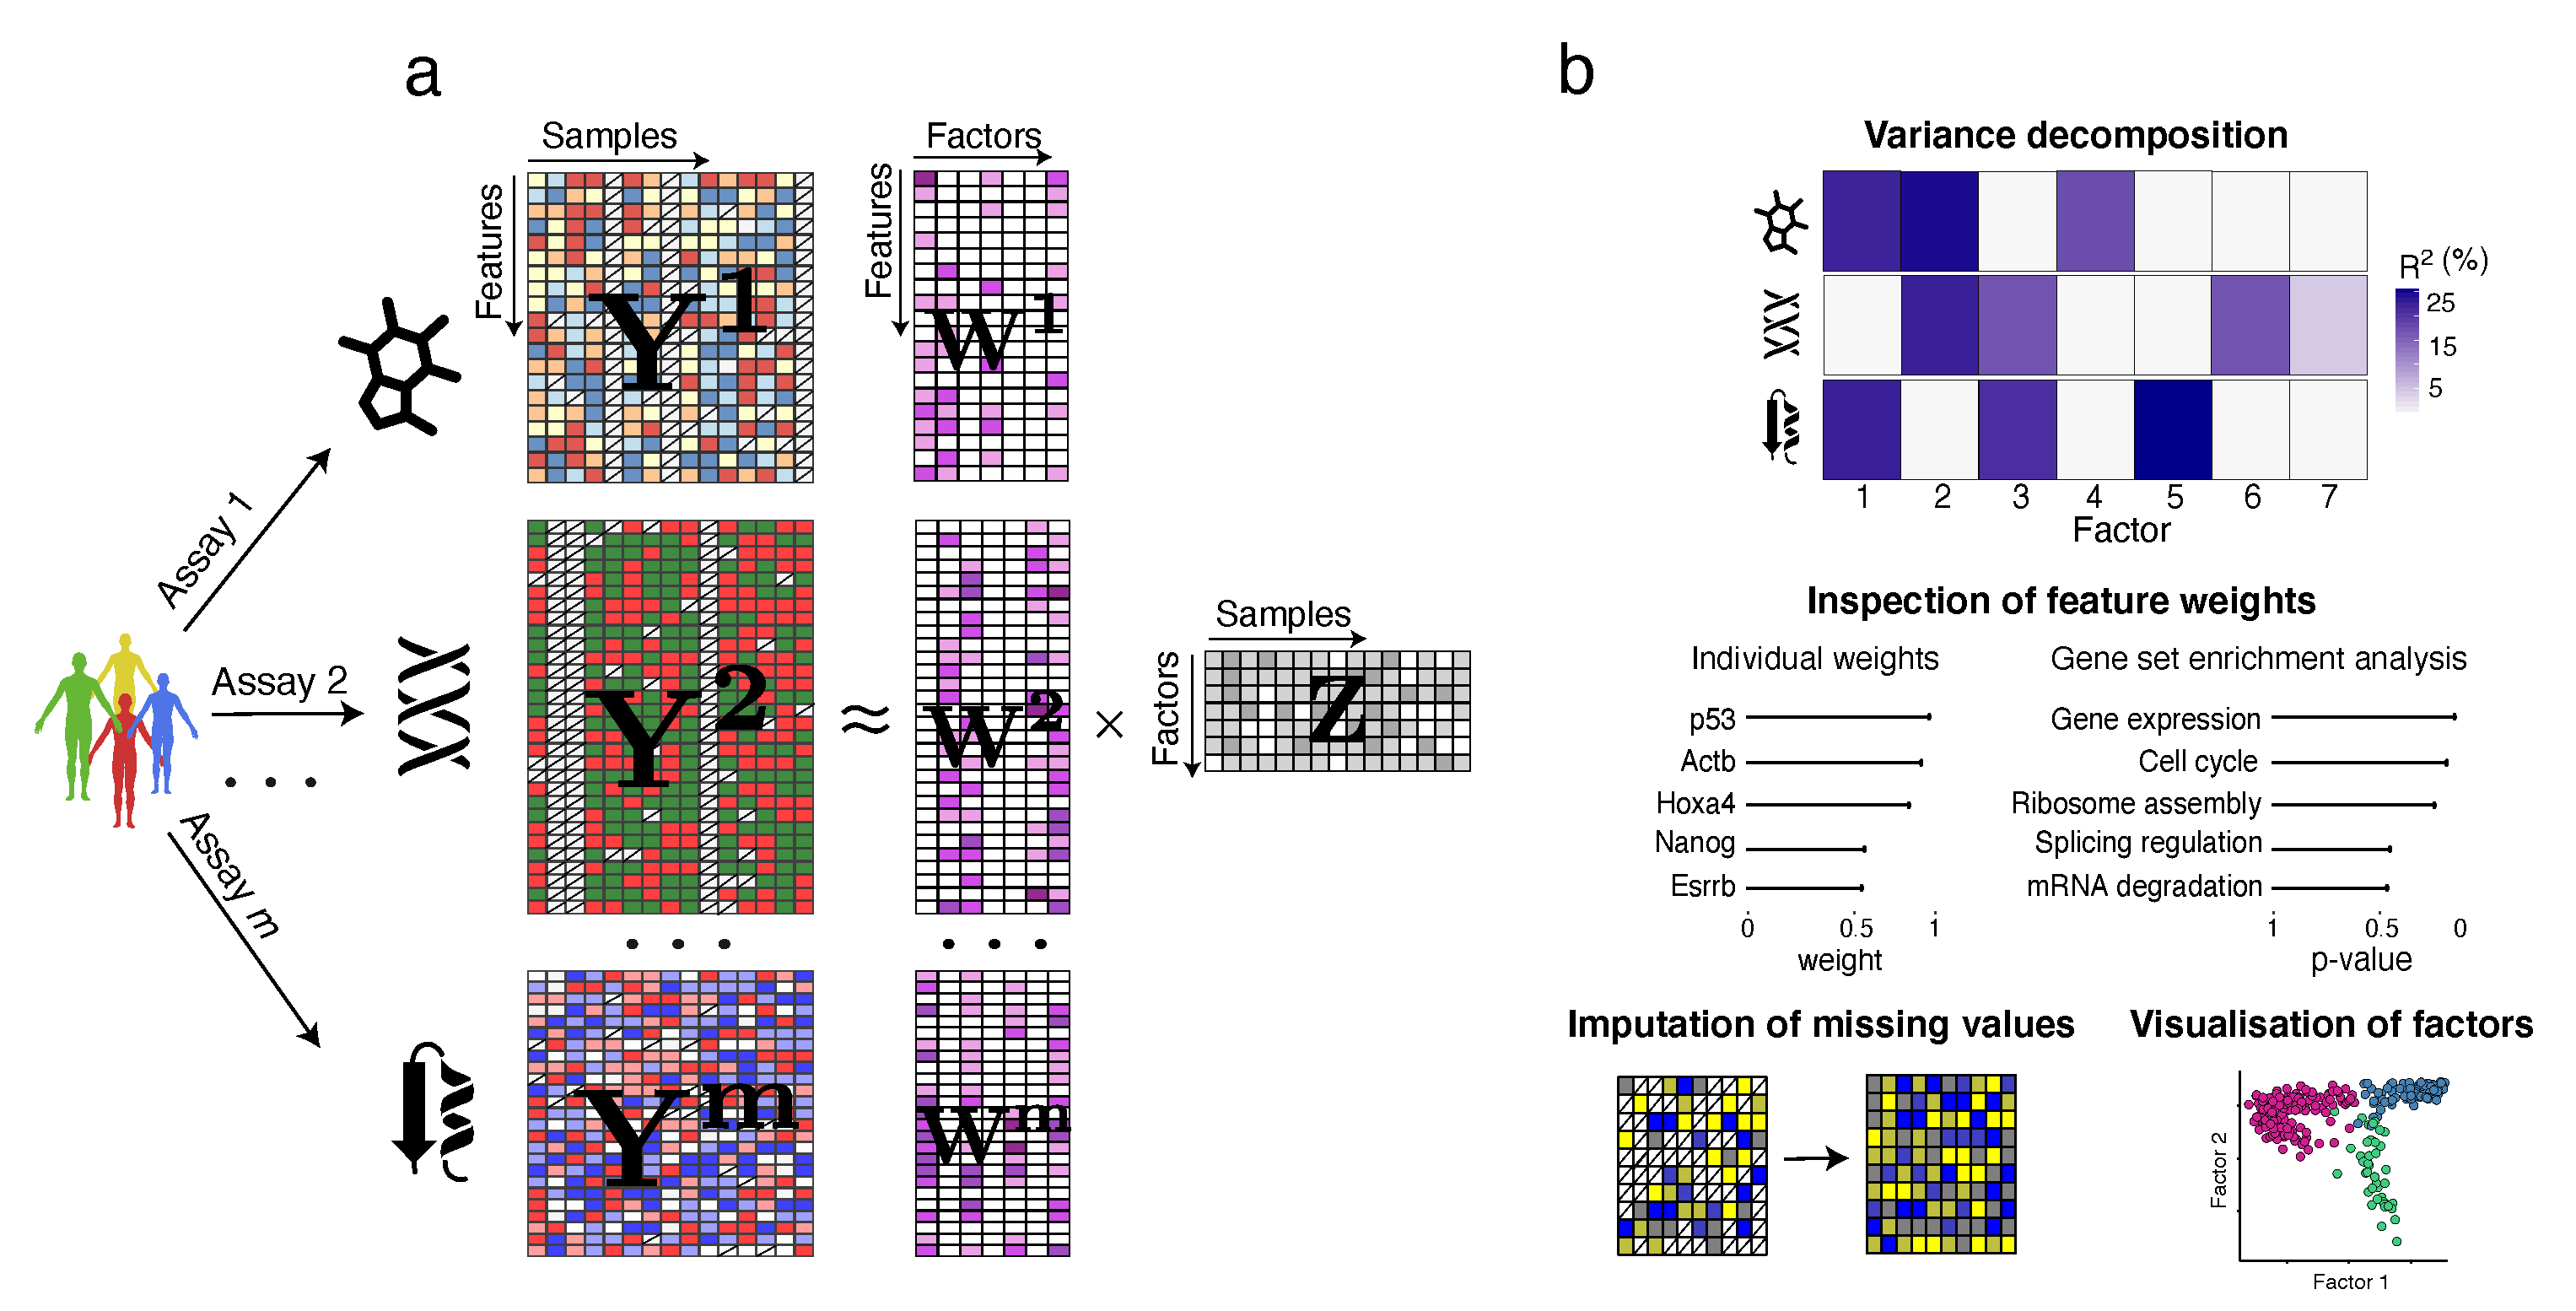
\includegraphics[width=1.0\textwidth]{MOFA}
		\caption{MOFA overview. The model takes $M$ data matrices as input ($\bfY^1, \cdots, \bfY^M$), one or more from each data modality, with co-occurrent samples but features that are not necessarily related and can differ in numbers. MOFA decomposes these matrices into a matrix of factors ($\bfZ$) and $M$ weight matrices, one for each data modality ($\bfW^1, \cdots, \bfW^M$). White cells in the weight matrices correspond to zeros, i.e. inactive features, whereas the cross symbol in the data matrices denotes missing values. The fitted MOFA model can be queried for different downstream analyses, including a variance decomposition to assess the proportion of variance explained by each factor in each data modality.}
		\label{fig:MOFA}
	\end{center}
\end{figure}

\begin{figure}[H]
	\centering
	% \definecolor{colD}{rgb}{0.2, 0.2, 0.6}
\definecolor{colM}{rgb}{0.0, 0.5, 0.0}
\definecolor{colN}{rgb}{0.5, 0.0, 0.13}
\definecolor{colG}{rgb}{1.0, 0.65, 0.0}
\newcommand\op{0.25}
\colorlet{shadecolor}{black!25}

\newcommand\op{0.25}

\begin{tikzpicture}
  % Define nodes:
  % matrix factorisation level
  \node[obs]   (Y) {$y_{n,d}^m$};
  \node[latent, above=of Y, xshift=-1.5cm] (Z) {$z_{n,k}$};
  \node[latent, above=of Y, xshift=1.5cm] (W) {$w_{k,d}^m$};
  \node[latent, xshift=1.5cm] (Tau) {$\tau_{d}^m$};

  % \node[opacity=\op,latent, xshift=-1.5cm] (Tau2) {$\tau_{n}$};

  % parents of Z
  \node[opacity=\op, det, above=of Z] (crossZ) {$\times$};
  \node[opacity=\op, latent, above=of crossZ] (Zhat) {$\hat{z}_{n,k}^{\ }$};
  \node[opacity=\op, latent, above=of Zhat] (SigmaZ) {$\alpha_k$};
  \node[opacity=\op, latent, above=of crossZ, xshift=-1.5cm] (SZ) {$s_{n,k}$};
  \node[opacity=\op, latent, above=of SZ] (ThetaZ) {$\theta_{k}$};

  % parents of W
  \node[det, above=of W] (crossW) {$\times$};
  \node[latent, above=of crossW] (What) {$\hat{w}_{k,d}^m$};
  \node[latent, above=of What] (SigmaW) {$\alpha_k^m$};
  \node[latent, above=of crossW, xshift=1.5cm] (SW) {$s_{k,d}^m$};
  \node[latent, above=of SW] (ThetaW) {$\theta_{k}^m$};

  % Connect the nodes
  \edge {Z,W, Tau} {Y}; %
  \edge[opacity=\op] {ThetaZ} {SZ};
  \edge[opacity=\op] {SigmaZ} {Zhat};
  \edge {ThetaW} {SW};
  \edge {SigmaW} {What};
  % \edge[opacity=\op] {Tau2} {Y}

  \factoredge[opacity=\op] {SZ, Zhat} {crossZ} {Z};
  \factoredge {SW, What} {crossW} {W};

  % cluster plate
  % \node[latent, above=of What, xshift=-1.3cm, opacity=0.15] (muW) {$\mu^m_{k, c}$};
  % \node[latent, above=of Zhat, xshift=1.3cm, opacity=0.15] (muZ) {$\mu_{k, c}$};
  % \edge[opacity=\op] {muZ} {Zhat};
  % \edge[opacity=\op] {muW} {What};
  % \plate[] {plateC} {(muZ)(muW)} {$C$};

  % Plates
  % \plate[] {plateK} {(Z)(W)(SZ)(Zhat)(SW)(What)(ThetaZ)(ThetaW)} {$K$};
  % \plate[color=colN, fill=colN, fill opacity=0.1] {plateN} {(Y)(Z)(crossZ)(Zhat)(SZ)(plateK.south west)} {\color{colN} $N$};
  % \plate[color=colD ,fill=colD, fill opacity=0.1] {plateD} {(Y)(W)(Tau)(crossW)(What)(SW)(plateK.south east) (plateN.south east)} {\color{colD}$D_m$};
  % \plate[color=colM,fill=colM, fill opacity=0.1] {plateM} {(plateD)(ThetaW)(plateK.north east)} {\color{colM}$M$};
  \plate[] {plateK} {(Z)(W)(SZ)(Zhat)(SW)(What)(ThetaZ)(ThetaW)} {$K$};
  \plate[] {plateN} {(Y)(Z)(crossZ)(Zhat)(SZ)(plateK.south west)} {$N$};
  \plate[] {plateD} {(Y)(W)(Tau)(crossW)(What)(SW)(plateK.south east) (plateN.south east)} {$D_m$};
  \plate[] {plateM} {(plateD)(ThetaW)(plateK.north east)} {$M$};

\end{tikzpicture}

	\caption{Graphical model for MOFA. The white circles represent hidden variables that are infered by the model, whereas the grey circles represent the observed variables. There are a total of four plates, each one representing a dimension of the model: $M$ for the number of views, $N$ for the number of samples, $K$ for the number of factors and $D_m$ for the number of features in the $m$-th view. The use of transparency in the top left nodes is intentional and becomes clear in Chapter 4 where we implement a spike-and-slab prior on the factors.}
	\label{fig:MOFA_graphical_model}
\end{figure}

\subsubsection{Inference}
To make the model scalable to large data sets we adopt a Variational inference framework with a structured mean field approximation. A detailed overview is given in \Cref{section:variational_inference}, and details on the variational updates for the MOFA model are given in Appendix XX.\\
To enable efficient inference for non-Gaussian likelihoods we employ local bounds \cite{Jaakkola2000,Seeger2012}. This is described in detail in \Cref{section:mofa_ngaussian}

\subsection{Monitoring convergence}
An attractive property of Variational inference is that the objective function, the Evidence Lower Bound (ELBO), increases monotonically at every iteration. This provides a simple way of monitoring convergence \Cref{fig:elbo_convergence}. This is indeed one of the reasons why we opted for this inference framework over Expectation Propagation or sampling-based approaches.

 \begin{figure}[H]
	\centering 	
	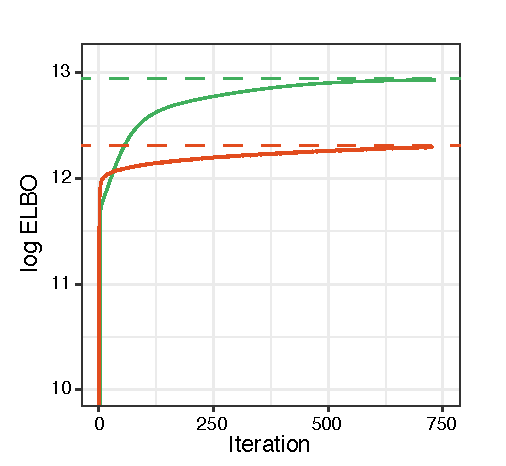
\includegraphics[width=0.5\textwidth]{elbo_convergence}
	\caption{Training curve for two diffent initialisations of MOFA. The y-axis displays the log of the ELBO, with higher values indicating a better fit. The x-axis displays the iteration number. The horizontal dash lines mark the value of the ELBO upon convergence. }
	\label{fig:elbo_convergence}
\end{figure}

\subsection{Model selection and consistency across random initilizations} \label{section:mofa_robustness}
The variational optimisation problem in MOFA is not convex and the posterior distributions will vary depending on the initialisation of the model. Thus, it becomes mandatory to perform model selection and assess the consistency of the factors across different trials.\\
The strategy we adopted in this work is to train several MOFA models (e.g. 10 trials) under different parameter initialisations, and after training we select the model with the highest ELBO for downstream analysis \Cref{fig:MOFA_robustness}. In addition, we evaluate the robustness of the factors by plotting the Pearson correlations between factors across all trials. \Cref{fig:MOFA_robustness}.\\
A similar strategy has also been proposed in \cite{Hore2016,Hore2015-thesis}.


\begin{figure}[H]
	\centering 	
	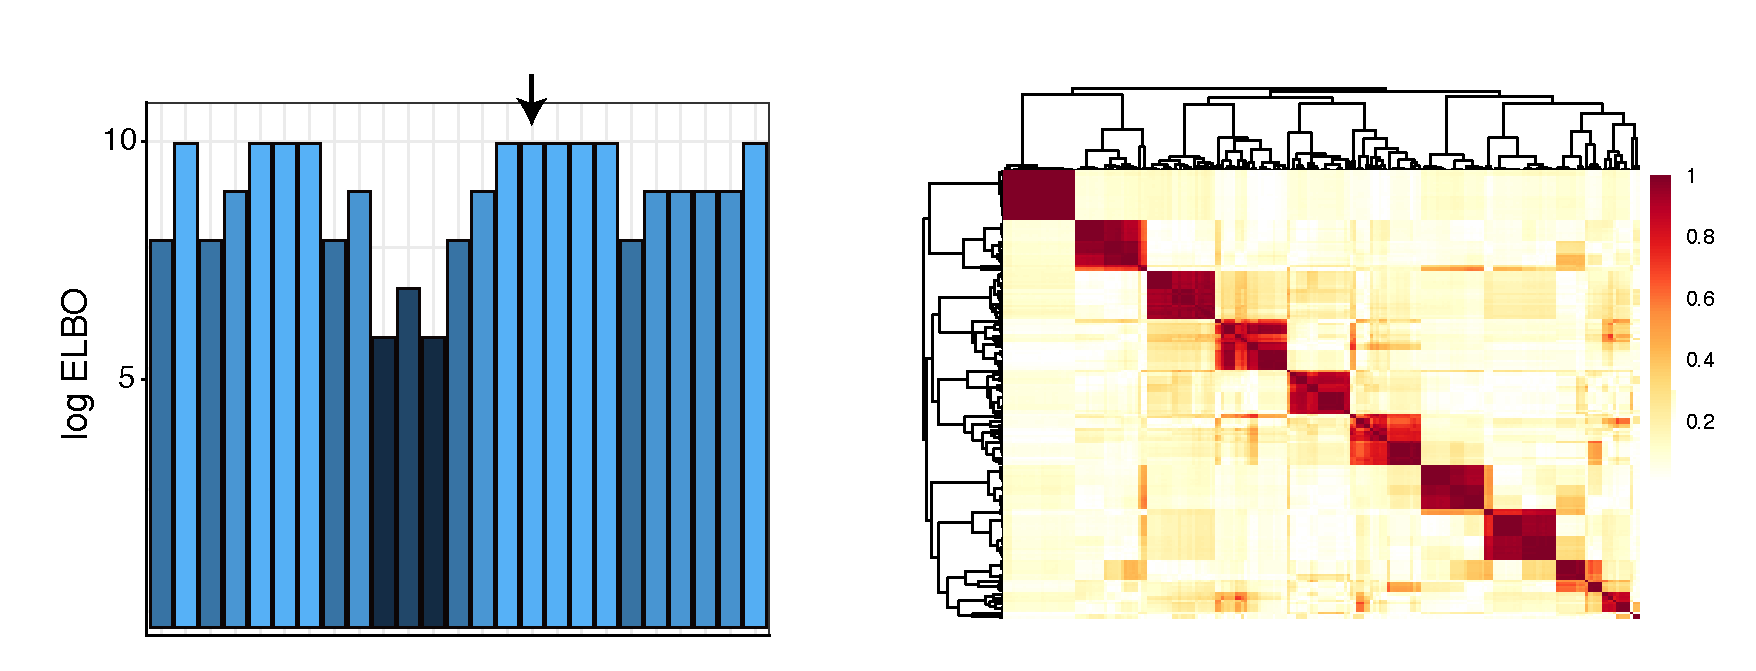
\includegraphics[width=1.0\textwidth]{MOFA_robustness}
	\caption{ Model selection and robustness analysis in MOFA. The left plot the log ELBO (y-axis) for 25 model instances (x-axis).
	The arrow indicates the model with the highest ELBO that would be selected for downstream analysis. The right plot displays the absolute value of the Pearson correlation coefficient between pairwise combinations of all factors across the 25 model instances. A block-diagonal matrix indicates that factors are robustly estimated regardless of the initialisation.}
	\label{fig:MOFA_robustness}
\end{figure}


% \subsection{Feature Set Enrichment Analysis}

% \subsection{Comparison with previous methods}

%The key difference with the sparse Bayesian factor analysis model in Section XX is that we learn a separate $\alpha_k^m$ and $\theta_k^m$ per factor and view, instead of per factor. This allows the model to take into account that the data is structured into different views.\\



\subsection{Learning the number of factors} \label{section:mofa_nfactors}
As described in section X, the use of an ARD prior allows factors to be actively prunned by the model if their variance explained is negligible. In the implementation we control the prunning of factors by a hyperparameter that defines a threshold on the minimum fraction of variance explained by a factor (across all views).\\
Additionally, because of the non-convexity of the optimisation problem, different model instances can potentially yield solutions with different number of active factors (\Cref{fig:mofa_nfactors}). Thus, the optimal number of factors can be selected by the model selection strategy outlined in \Cref{section:robustness}.

\begin{figure}[H]
	\centering 	
	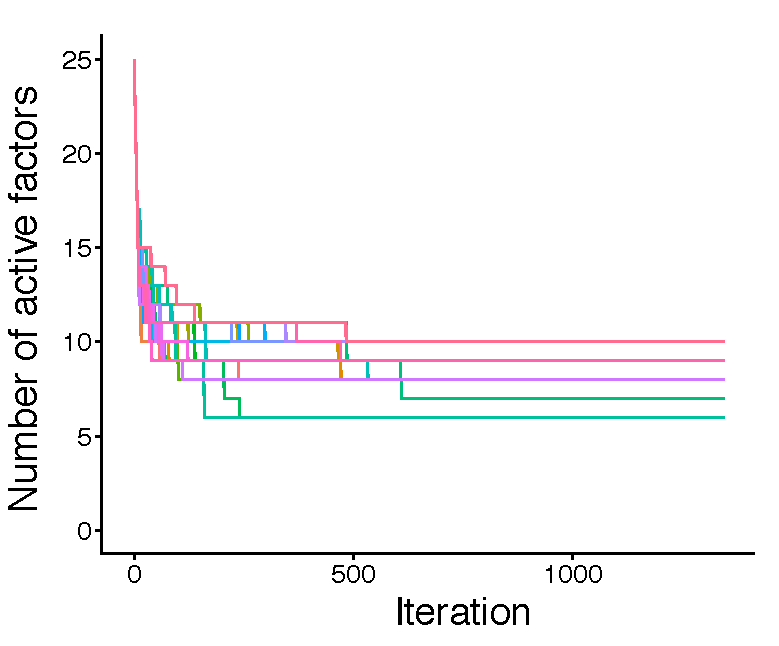
\includegraphics[width=0.5\textwidth]{MOFA_nfactors}
	\caption{Training curve for the number of active factors across 25 different model instances. The y-axis displays the number of active factors. The x-axis displays the iteration number. Different lines denote different model instances.}
	\label{fig:MOFA_nfactors}
\end{figure}


\subsection{Modelling and inference with non-Gaussian data} \label{section:mofa_ngaussian}
To implement efficient variational inference in conjunction with a non-Gaussian likelihood we adapt prior work from \cite{Seeger2012} using local variational bounds. The key idea is to dynamically approximate non-Gaussian data by Gaussian pseudo-data based on a second-order Taylor expansion.  To make the approximation justifiable we need to introduce variational parameters that are adjusted alongside the updates to improve the fit.	\\
Denoting the parameters in the MOFA model as $\bfX= (\bfZ,\bfW,\balpha,\btau,\btheta)$, recall that the variational framework approximates the posterior $p(\bfX | \bfY )$ with a distribution $q(\bfX)$, which is indirectly optimised by optimising a lower bound of the log model evidence. The resulting optimization problem can be re-written as
\begin{equation*}
\min_{q(\bfX)} -\Lagr(\bfX) =  \min_{q(\bfX)} \E_q \big[ -\log p(\bfY|\bfX) \big] + \KL[q(\bfX)||p(\bfX)].
\end{equation*}


Expanding the MOFA model to non-Gaussian likelihoods we now assume a general likelihood of the form $p(\bfY|\bfX)=p(\bfY|\bfC)$ with $\bfC = \bfZ\bfW^{T}$, that can write as

\begin{equation*}
-\log p(\bfY|\bfX) = \sum_{n=1}^{N} \sum_{d=1}^{D} f_{nd} (c_{nd})
\end{equation*}
with $f_{nd}(c_{nd}) = -\log p(y_{nd}|c_{nd})$. We dropped the view index $m$ to keep notation uncluttered.\\
Extending \cite{Seeger2012} to our heteroscedastic noise model, we require $f_{nd}(c_{nd})$ to be twice differentiable and bounded by $\kappa_d$, such that $f_{nd}''(c_{nd}) \leq \kappa_d \,\forall n,d$. This holds true in many important models as for example the Bernoulli and Poisson case. Under this assumption a lower bound on the log likelihood can be constructed using Taylor expansion,
\begin{equation*}
f_{nd}(c_{nd}) \leq \frac{\kappa_d}{2} (c_{nd} - \zeta_{nd})^2 + f'(\zeta_{nd})(c_{nd} - \zeta_{nd}) + f_{nd}(\zeta_{nd}) := q_{nd}(c_{nd},\zeta_{nd}),
\end{equation*}
where $\bZeta =  \zeta_{nd} $ are additional variational parameters that determine the location of the Taylor expansion and have to be optimised to make the lower bound as tight as possible. Plugging the bounds into above optimization problem, we obtain:
\begin{equation*}
\min_{q(\bfX),\bZeta} \quad \sum_{d=1}^{D}\sum_{n=1}^{N} \E_q [ q_{nd}(c_{nd},\zeta_{nd})] + \KL[q(\bfX)||p(\bfX)]
\end{equation*}
The algorithm propsed in \cite{Seeger2012} then alternates between updates of $\bZeta$ and $\mathrm{q}(\bTheta)$. The update for $\bZeta$ is given by
\begin{equation*}
\zeta \leftarrow \E[\bfW]\E[\bfZ]^{T}
\end{equation*}
where the expctations are taken with respect to the corresponding $q$ distributions.\\
% In order to find the updates for $q(\bTheta)$ we bring the taylor approximation of $q(f_{nd})$ in q audratic form:
% \begin{equation*}
% q(f_{nd},\zeta_{nd}) \propto \frac{\kappa_d}{2}(f_{nd} - (zeta_{nd} - g(\zeta_{nd})/\kappa_d))^2
% \end{equation*}
% and note that this is proportional to the log of a Gaussian distribution $-log \Normal (\hat{y}_{nd}|f_{ng},\frac{1}{ng})$ where $\hat{y}_{nd} = zeta_{nd} - g'(\zeta_{nd})/\kappa_d$ is defined as a pseudodata based on the zero-inflated observations.
% Consequently, for fixed $\zeta_{nd}$, the updates of the variational distributions $Q(X)$ and $Q(W)$ are equivalent to the ones derived in X, but with pseudodata $\hat{Y}$ and precision $\kappa_g$
On the other hand, the updates for $q(\bfX)$ can be shown to be identical to the variational Bayesian updates with a conjugate Gaussian likelihood when replacing the observed data $\bfY$ by a pseudo-data $\hat{\bfY}$ and the precisions $\tau_{nd}$ (which were treated as random variables) by the constant terms $\kappa_d$ introduced above.\\
The pseudodata is given by
\begin{equation*}
\hat{y}_{nd} = \zeta_{nd} - f'(\zeta_{nd})/\kappa_d.
\end{equation*}
Depending on the log likelihoods $f(\cdot)$ different $\kappa_d$ are used resulting in different pseudo-data updates. Two special cases implemented in MOFA are the Poisson and Bernoulli likelihood described in the following.

\subsubsection*{Bernoulli likelihood for binary data}
When the observations are binary, $y \in \{0,1\}$, they can be modelled using a Bernoulli likelihood:
%\begin{equation*}
%p(y|c) = \frac{e^{yc}}{1+e^c}
%\end{equation*}
%The second derivative of the log likelihood is bounded by:
%\begin{equation*}
%f''(c) = \sigma(c)\sigma(-c) \leq 1/4 := \kappa
%\end{equation*}
%where $\sigma$ is the sigmoid function $f(c) = 1/(1+e^{-c})$.\\
%The pseudodata updates are given by
%\begin{equation*}
%\hat{y}_{nd} = \zeta_{nd} - 4*(\sigma(\zeta_{nd}) - y_{nd})
%\end{equation*}
\begin{equation*}
\bfY|\bfZ,\bfW \sim \text{Ber}(\sigma(\bfZ\bfW^T)),
\end{equation*} where $\sigma(a)=(1+e^{-a})^{-1}$ is the logistic link function and $\bfZ$ and $\bfW$ are the latent factors and weights in our model, respectively.\\
In order to make the variational  inference efficient and explicit as in the Gaussian case, we aim to approximate the Bernoulli data by a Gaussian pseudo-data as proposed in \cite{Seeger2012} and described above which allows to recycle all the updates from the model with Gaussian views. While \cite{Seeger2012} assumes a homoscedastic approximation with a spherical Gaussian, we adopt an approach following \cite{Jaakkola2000}, which allows for heteroscedaticity and provides a tighter bound on the Bernoulli likelihood.\\
Denoting $c_{nd}=(\bfZ\bfW^T)_{nd}$ the Jaakkola upper bound \cite{Jaakkola2000} on the negative log-likelihood is given by
\begin{align*}
\begin{split}
-\log\left(p(y_{nd}|c_{nd})\right) &= -\log\left(\sigma\left((2y_{nd}-1)  c_{nd}\right)\right)\\
& \leq -\log(\zeta_{nd})-\frac{(2y_{nd}-1)c_{nd}-\zeta_{nd})}{2} +\lambda(\zeta_{nd})\left(c_{nd}^2 -\zeta_{nd}^2 \right)\\
& =: b_J(\zeta_{nd}, c_{nd},y_{nd} )
\label{jaakkola}
\end{split}
\end{align*}
with $\lambda$ given by $\lambda(\zeta)=\frac{1}{4\zeta}\tanh\left(\frac{\zeta}{2}\right)$.\\
This can easily be derived from a first-order Taylor expansion on the function $f(x) = - \log(e^{\frac{x}{2}}+e^{-\frac{x}{2}}) = \frac{x}{2}-\log(\sigma(x))$ in $x^2$ and by the convexity of 
$f$ in $x^2$ this bound is global as discussed in \cite{Jaakkola2000}.\\
In order to make use of this tighter bound but still be able to re-use the variational updates from the Gaussian case we re-formulate the bound as a Gaussian likelihood on pseudo-data $\hat{\bfY}$.\\
As above we can plug this bound on the negative log-likelihood into the variational optimization problem to obtain  \begin{equation*}
\min_{q(\bfX),\bZeta} \quad \sum_{d=1}^{D}\sum_{n=1}^{N} \mathbb{E}_q b_J(\zeta_{nd}, c_{nd},y_{nd} ) + \KL[q(\bfX)||p(\bfX)].
\end{equation*}
This is minimized iteratively in the variational parameter $\zeta_{nd}$ and the variational distribution of Z,W:\\
Minimizing in the variational parameter $\zeta$ this leads to the updates given by
\begin{equation*}
\zeta_{nd}^2 = \mathbb{E}[c_{nd}^2]
\end{equation*}
as described in \cite{Jaakkola2000}, \cite{Bishop}.\\
For the variational distribution $q(\bfZ,\bfW)$ we observe that the Jaakkola bound can be re-written as 
\begin{equation*}
b_J(\zeta_{nd}, c_{nd},y_{nd} ) = -\log\left(\varphi\left(\hat{y}_{nd}; c_{nd}, \frac{1}{2\lambda(\zeta_{nd})}\right)\right) + \gamma(\zeta_{nd}),
\end{equation*}
where $\varphi(\cdot; \mu, \sigma^2)$ denotes the density function of a normal distribution with mean $\mu$ and variance $\sigma^2$ and $\gamma$ is a term only depending on $\bZeta$. This allows us to re-use the updates for $\bfZ$ and $\bfW$ from a setting with Gaussian likelihood by considering the Gaussian pseudo-data 
\begin{equation*}
\hat{y}_{nd}= \frac{2y_{nd}-1}{4 \lambda(\zeta_{nd})}
\end{equation*}
updating the data precision as $\tau_{nd} = 2\lambda(\zeta_{nd})$ using  updates generalized for sample- and feature-wise precision parameters on the data.


\subsubsection*{Poisson likelihood for count data}
When observations are a natural numbers, such as count data $y \in \N = \{0,1,\cdots\}$, they can be modelled using a Poisson likelihood:
\begin{equation*}
p(y|c) = \lambda(c)^y e^{-\lambda(c)}
\end{equation*}
where $\lambda(c)>0$ is the rate function and has to be convex and log-concave in order to ensure that the likelihood is log-concave.\\
As done in \cite{Seeger2012}, here we choose the following rate function: $\lambda(c)=\log(1+e^c)$.

Then an upper bound of the second derivative of the log-likelihood is given by
\begin{equation*}
f''_{nd}(c_{nd}) \leq \kappa_d = 1/4 + 0.17*\max(\bfy_{:,d}).
\end{equation*}
%The bound degrades with the presence of entries with large values. Thus, we follow common practice and clip overly large counts.\\
The pseudodata updates are given by
\begin{equation*}
\hat{y}_{nd} = \zeta_{nd} - \frac{\mathrm{S}(\zeta_{nd})(1-y_{nd}/\lambda(\zeta_{nd}))}{\kappa_d}.
\end{equation*}


\subsection{Model validation with simulated data} \label{section:mofa_simulated}
We used simulated data from the generative model to systematically test the technical capabilities of MOFA.





\subsubsection{Recovery of the latent space}
First, we tested the ability of MOFA to recover simulated factors, varying the number of views, the number of features, the number of factors and the fraction of missing values.\\ 
For every simulation scenario we initialised a model with a high number of factors ($K=100$), and inactive factors were automatically dropped during model training using a threshold of 1\% variance explained. In addition, to test the robustness under different initialisations, ten models were trained for every simulation scenario.\\
We observe that in most settings the model accurately recovers the correct number of factors (\Cref{fig:MOFA_learnK}). Exceptions occur when the dimensionality of the latent space is too large (more than 50 factors) or when an excessive amount of missing values (more than 80\%) is present in the data.

\begin{figure}[H]
	\centering 	
	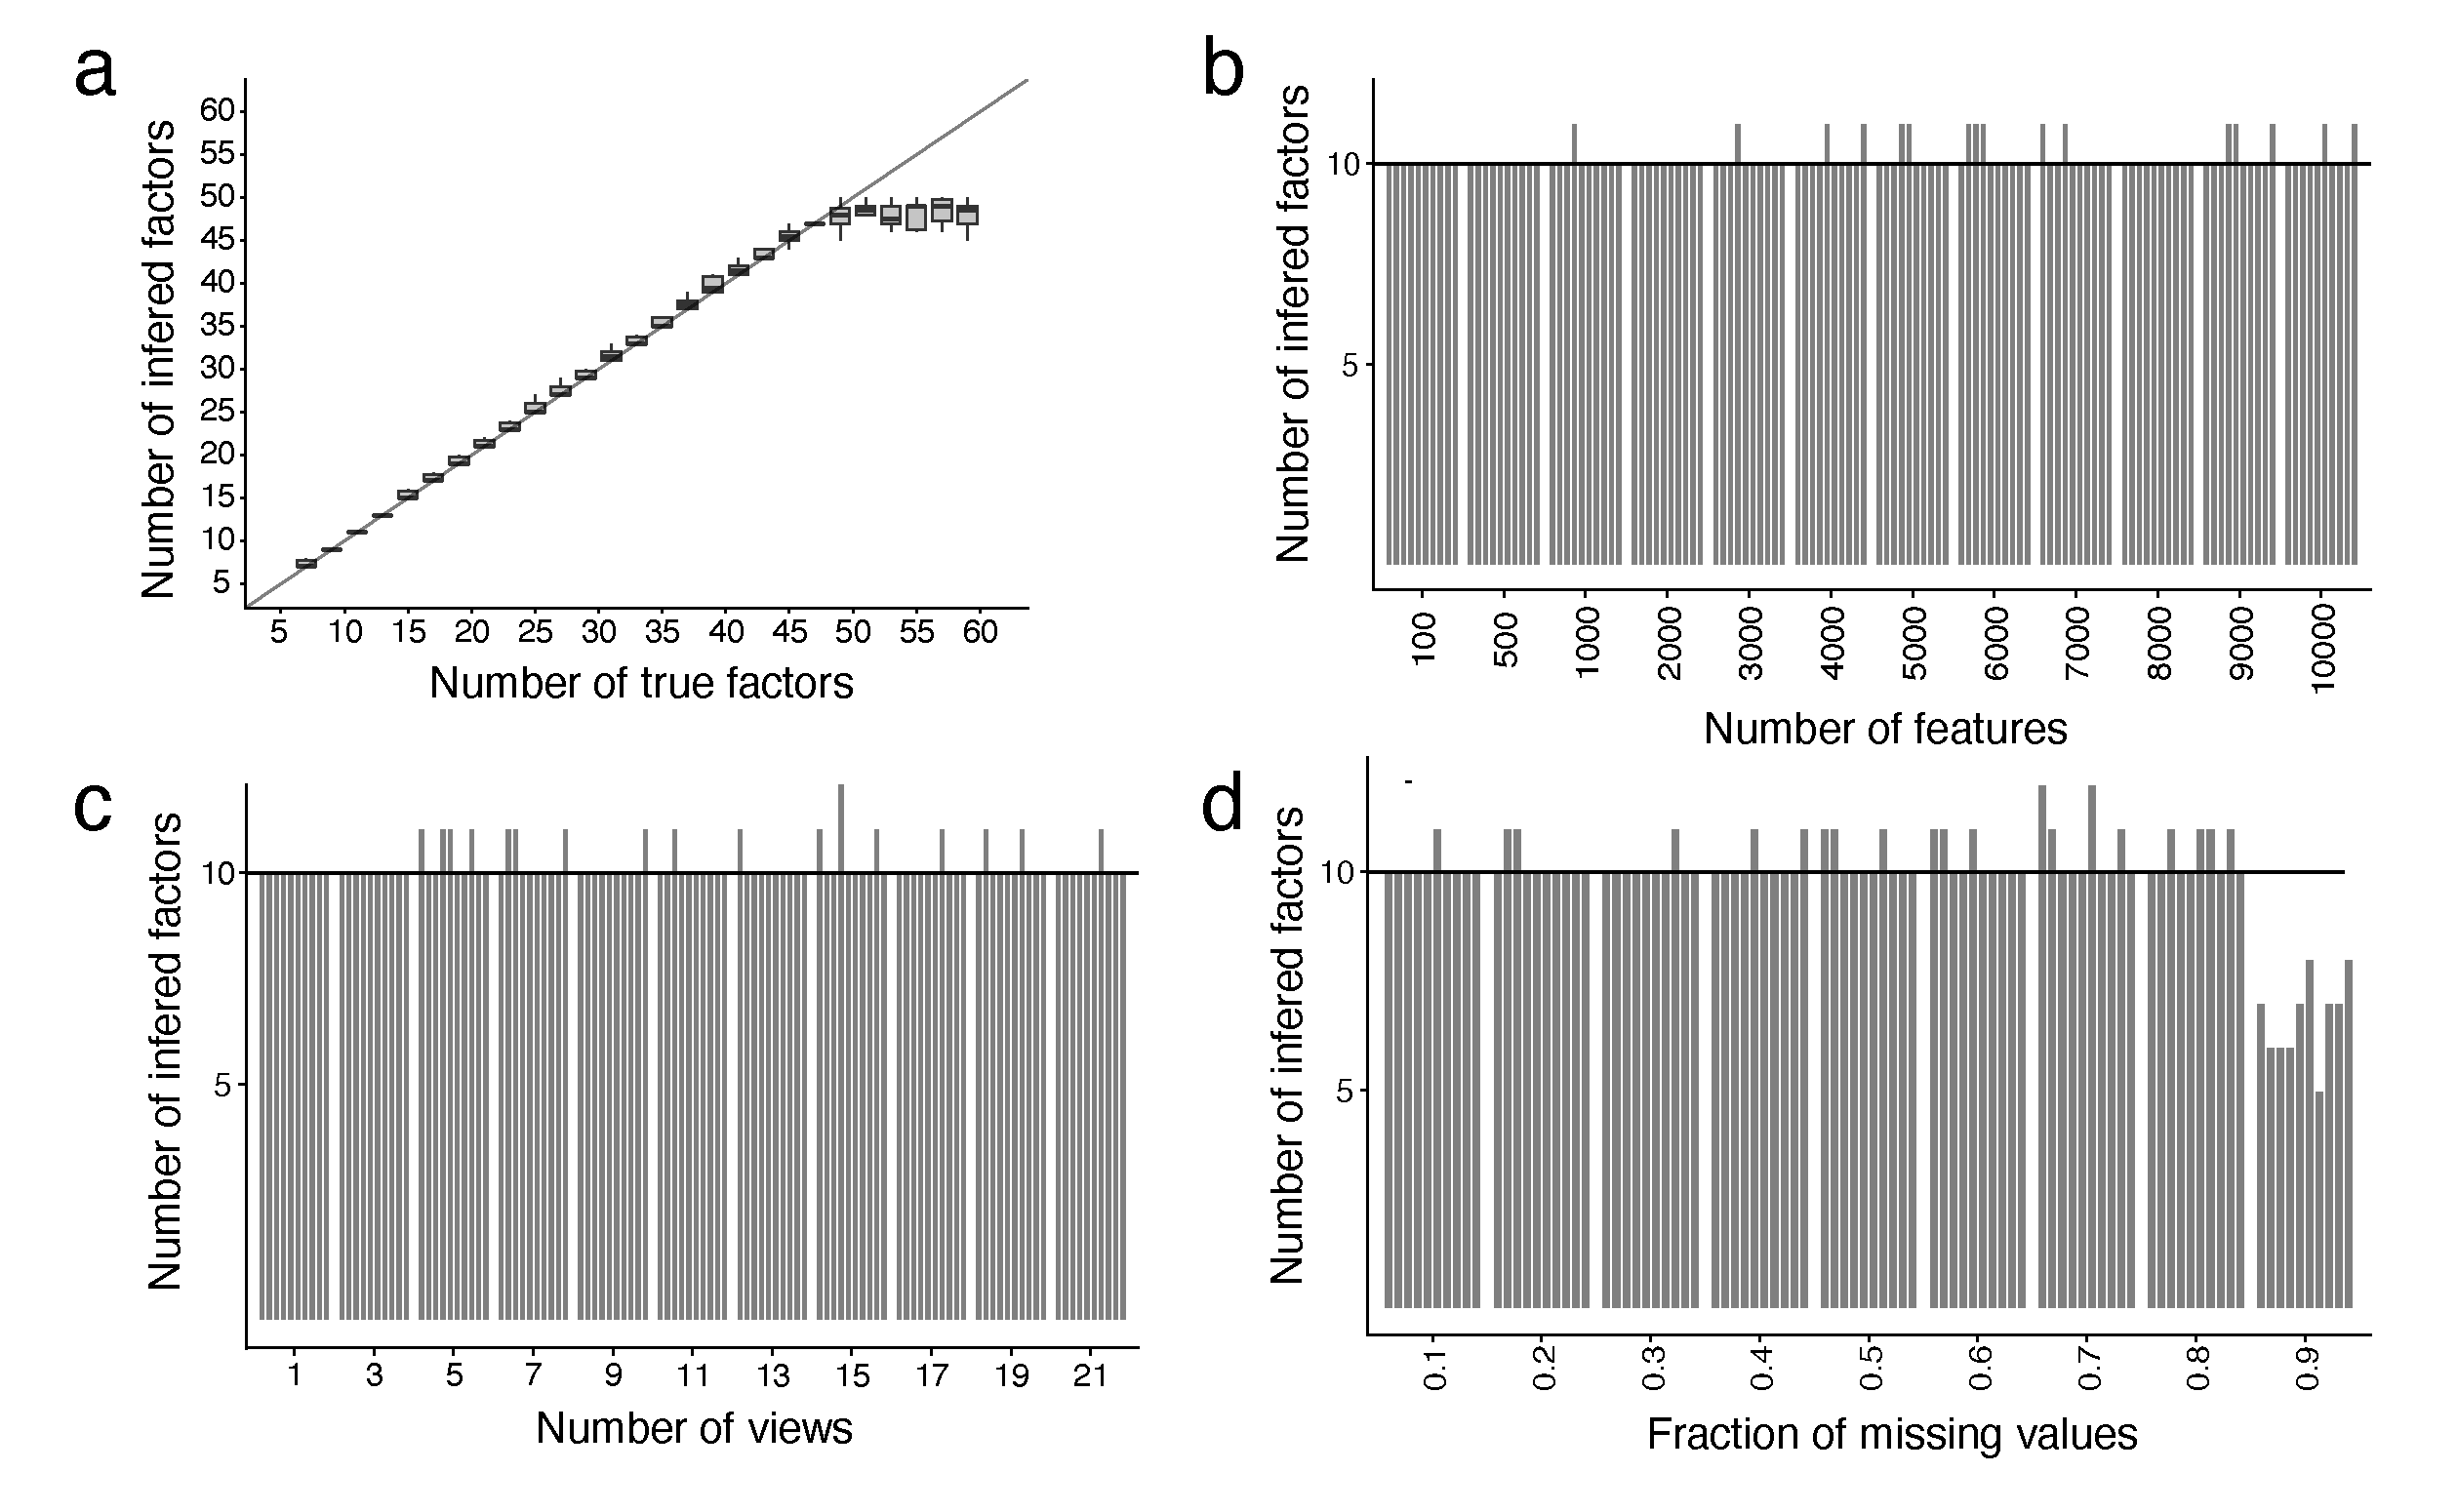
\includegraphics[width=1.0\textwidth]{MOFA_learnK}
	\caption{Assessing the ability of MOFA to recover simulated latent spaces. In all plots the y-axis displays the number of infered factors. (a) x-axis displays the number of true factors, and boxplots summarise the distribution across 10 model instances. For (c-d) the true number of factors was set to $K=10$ and each bar corresponds to a different model instance. (b) x-axis displays the number of features, (c) x-axis displays the number of views, (d) x-axis displays fraction of missing values. }
	\label{fig:MOFA_learnK}
\end{figure}

\subsubsection{Group-wise sparsity on the loadings}
One of the most important statistical assumptions underlying MOFA (and other Group Factor Analysis methods) is the sparsity prior aimed at disentangling the activity of factors across views.\\
To evaluate this feature we simulated data from the generative model were the factors were clearly set to be active or inactive in specific views. We compared the performance with two other methods: the iCluster+ model \cite{Mo2013} and a GFA implementation \cite{Leppaaho2017}.\\
the GFA implementation shares the same factor and view-wise sparsity as MOFA, and is therefore expected to show similar performance. On the other hand, iCluster is a model that is aimed at clustering and it only contains a sparsity constraint (in a penalised maximum likelihood setting) per factor, shared across all views.\\
On simulated data, MOFA and GFA correctly infer the true activity pattern of the factors whereas iCluster infers incorrect sharedness of factors across views, especially with increasing dimensionality of the latent space.

\begin{figure}[H]
	\centering 	
	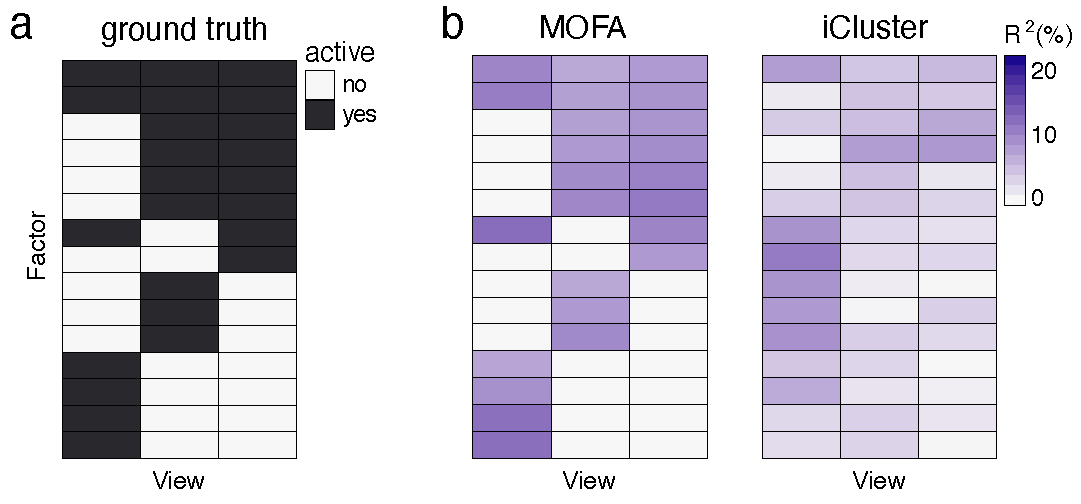
\includegraphics[width=1.0\textwidth]{MOFA_group_sparsity}
	\caption{Evaluating the ability of MOFA, iCluster and GFA to recover sparse factor activity patterns across views. The leftmost plot displays the true activity pattern, with factors being (strongly) active in different subsets of views. The remaining three plots show, for each model, the fraction of variance explained ($R^2$) by each factor in each view.}
	\label{fig:MOFA_group_sparsity}
\end{figure}

\subsubsection{Feature-wise sparsity on the loadings}
A key aspect of MOFA is the use of a spike-and-slab prior distribution to enforce feature-wise sparsity on the loadings, which yields a more interpretable solution (see \Cref{section:mofa_priors}).\\
To assess the effect of the spike-and-slab prior we fit a group of models with a spike-and-slab prior and another group of models only with Automatic Relevance Determination prior. We further compared both solutions to a conventional Principal Component Analysis fit on the concatenated data set.\\
As expected, we observe that the spike-and-slab prior induces more zero-inflated weights, although the ARD prior provided a moderate degree of regularisation. The PCA solution was notably more dense than both bayesian models (\Cref{fig:MOFA_sparsity}).

\begin{figure}[H]
	\centering 	
	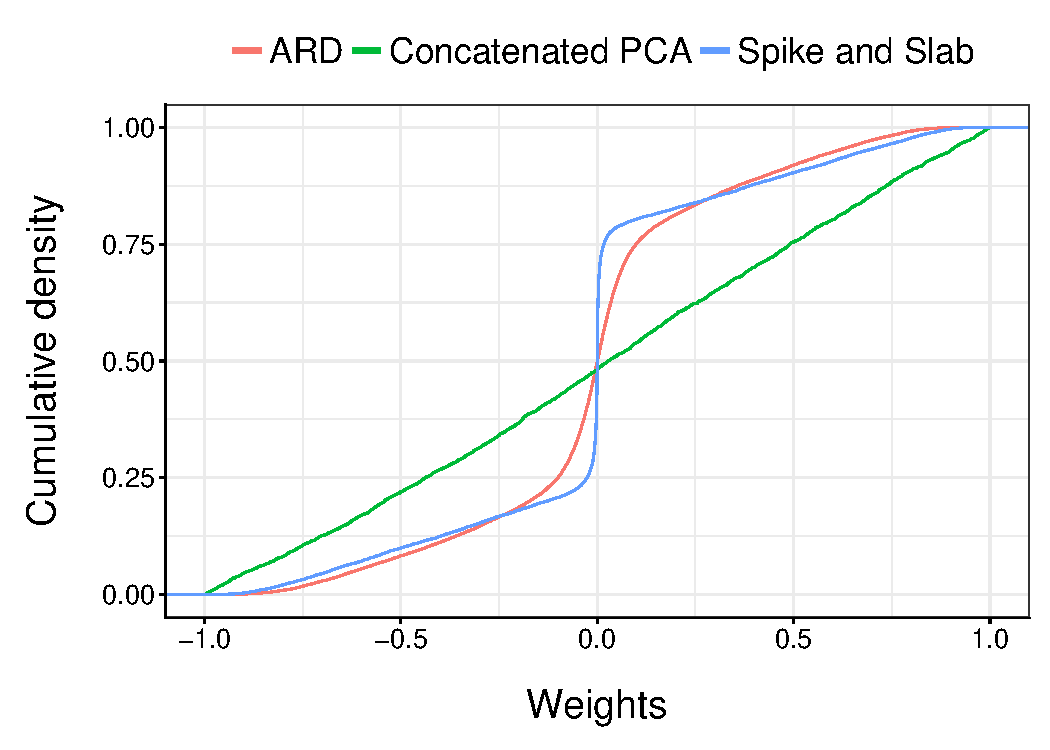
\includegraphics[width=0.7\textwidth]{MOFA_sparsity}
	\caption{Assessing sparsity on the loadings in MOFA. The plot shows the empirical cumulative density function of the loadings for an arbitrary factor in a single view. The loadings were simulated with a sparsity level of $\theta_k^m=0.5$ (50\% of active features.)
	}
	\label{fig:MOFA_sparsity}
\end{figure}


\subsubsection{Non-gaussian likelihoods}  \label{section:mofa_nongaussian_results}
A key improvement of MOFA with respect to previous methods is the use of non-Gaussian likelihoods to integrate multiple data modalities. As described in \Cref{section:mofa_ngaussian}, we implemented a Bernoulli likelihood to model binary data and a Poisson likelihood to model count data.\\
To validate both likelihood models, we simulated binary and count data using the generative model and we fit two sets of models for each data type: a group of models with a Gaussian likelihood and a group of models with a Bernoulli or Poisson likelihood, respectively.\\
We observe that although both likelihoods are able to recover the true number of factors, the models with the non-Gaussian likelihoods clearly result in a better fit to the data (\Cref{fig:MOFA_nongaussian_binary,fig:MOFA_nongaussian_poisson}).

\begin{figure}[H]
	\centering 	
	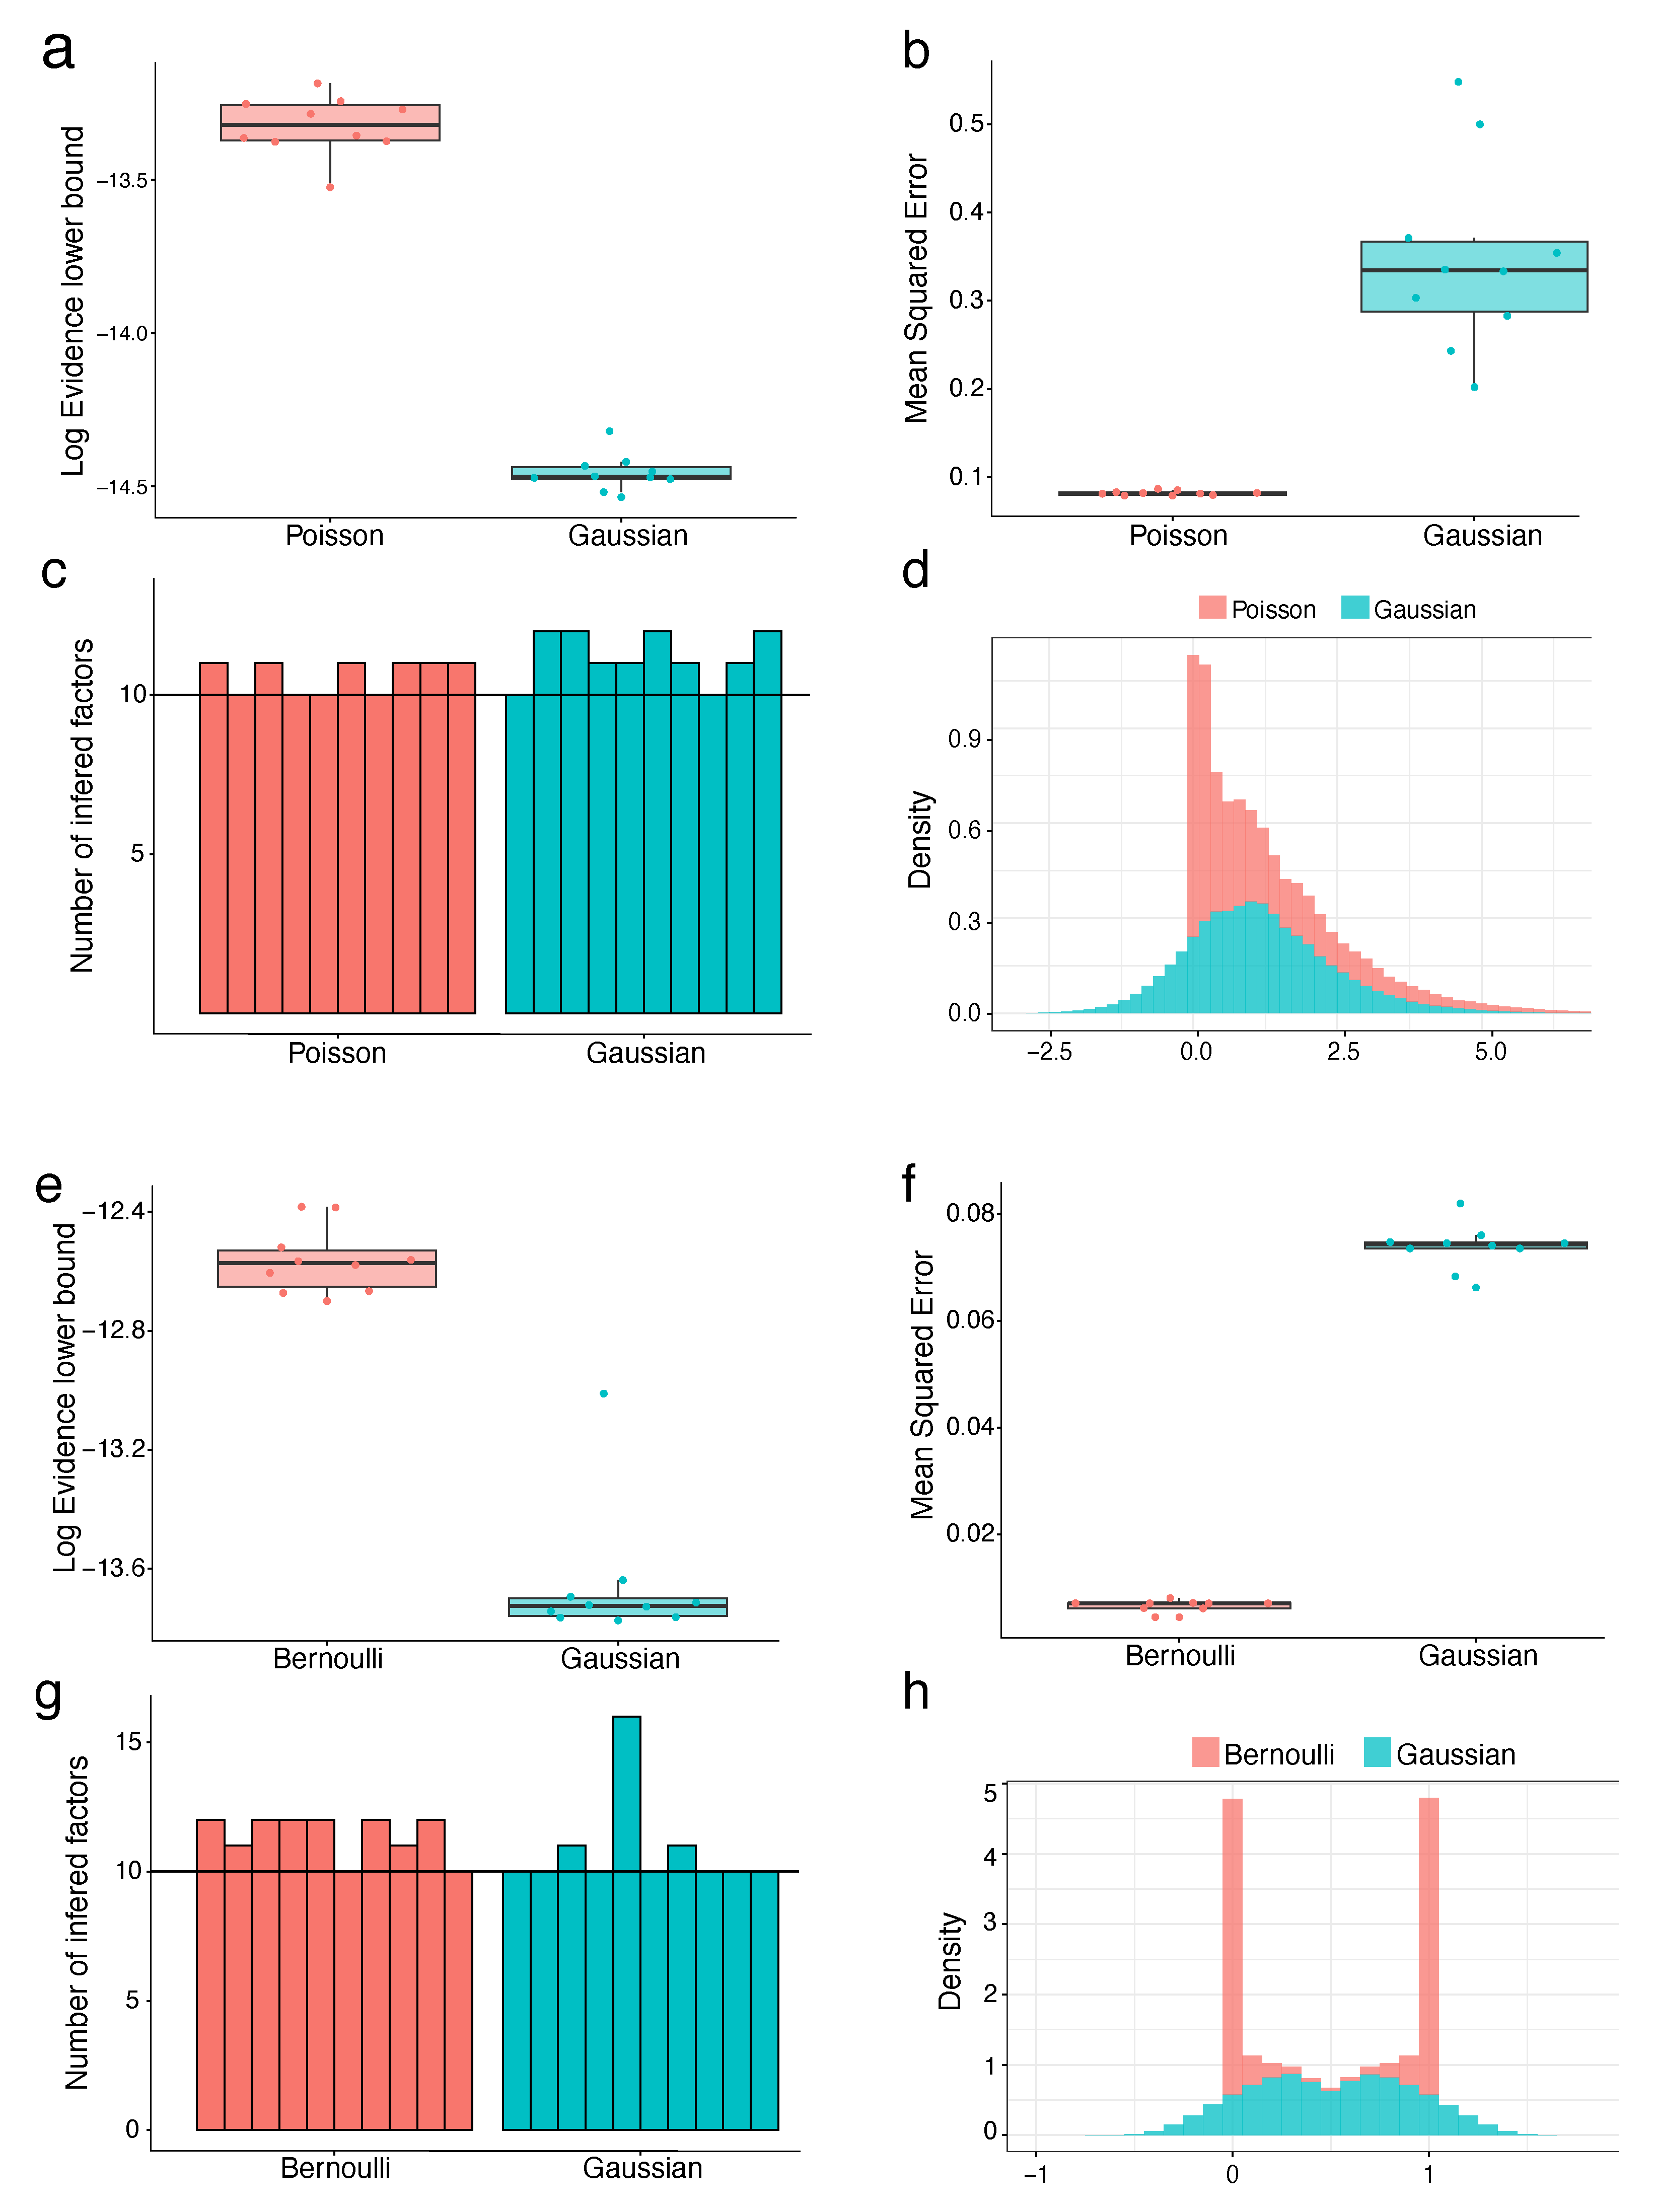
\includegraphics[width=1.0\textwidth]{MOFA_nongaussian}
	\caption{Validation of the non-gaussian likelihood models implemented in MOFA on simulated data. The four plots on the left assess the Poisson and the Gaussian likelihoods applied to count data. The four plots on the right assess the Bernoulli and the Gaussian likelihoods applied to binary data. (a) The y-axis displays the ELBO for each model instance (x-axis). (b) The y-axis displays the mean reconstruction error for each model instance (x-axis). (c) The y-axis displays the number of estimated factrors for each model instance (x-axis). The horizontal dashed line marks the true number of factors $K=10$. (d) Distribution of reconstructed data.}
	\label{fig:MOFA_nongaussian}
\end{figure}


\subsubsection{Scalability}
Finally, we evaluated the scalability of the model when varying each of its dimensions independently (\Cref{fig:MOFA_scalability}), and we compared the speed with a Gibbs sampling implementation of GFA \cite{Leppaaho2017} and iCluster+ \cite{Mo2013}.\\
Overall, we observe that MOFA scales linear with respect to all dimensions and is significantly faster than any of the three evaluated techniques.\\
As a real application showcase, the training on the CLL data \Cref{fig:MOFA_CLL_Figure1} required 25 minutes using MOFA, 34 hours with GFA and 5-6 days with iCluster.

\begin{figure}[H]
	\centering 	
	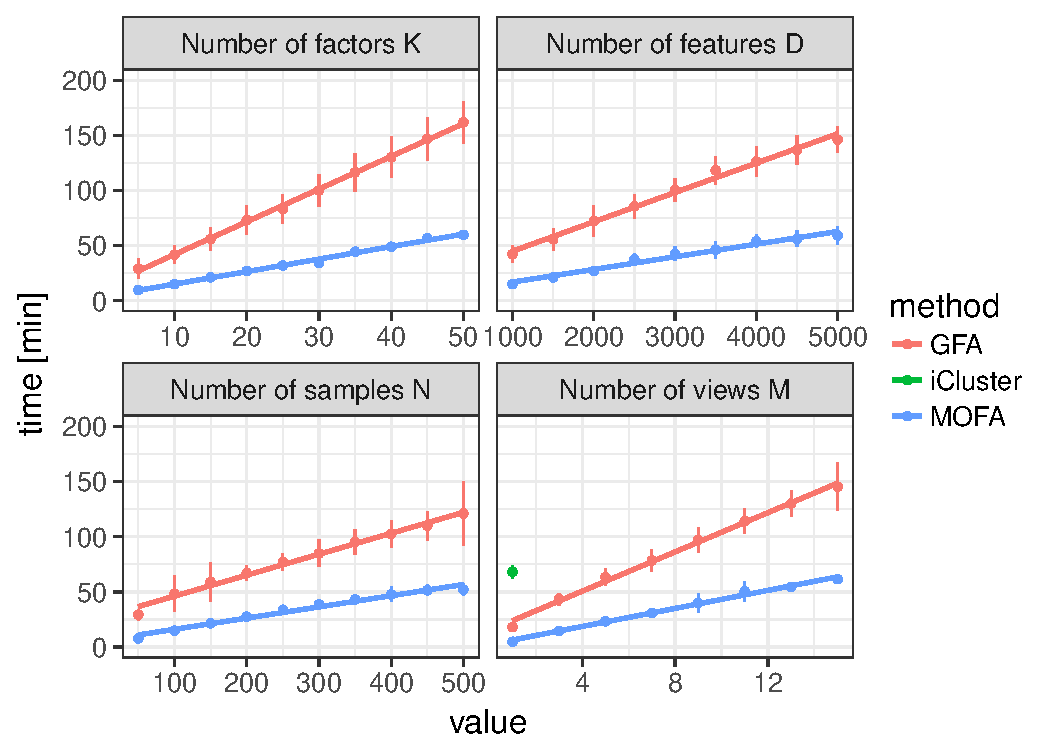
\includegraphics[width=0.9\textwidth]{MOFA_scalability}
	\caption{Evaluation of speed and scalability in MOFA. The y-axis displays the time required for convergence. The x-axis displays the value of the dimension that was tested, either number of factors ($K$), number of features ($D$), number of samples ($N$) and number of views ($M$). Baseline parameters were $M=3, K=10, D=1000, N=100$. Each line represents a different model, GFA (red), MOFA (blue) and iCluster (green). Default convergence criteria where used for all methods. Each dot displays the average time across 10 trials with error bars denoting the standard deviation. iCluster is only shown for one value as all other settings required more than 200min for convergence.
	}
	\label{fig:MOFA_nongaussian}
\end{figure}



\subsection{Application to chronic lymphocytic leukaemia} \label{section:mofa_cll}
Personalised medicine is an attractive field for the use of multi-omics, as dissecting heterogeneity across patients is a major challenge in complex diseases, and requires integration of information from multiple biological layers \cite{Chen2013,Costello2014,Alyass2015}.\\
In most cases, predicting patient survival and response to a treatment is still not reliable due to a lack of predictive biomarkers and our incomplete understanding of the mechanisms underlying response heterogeneity. Identification of the main drivers of inter-patient variation and their molecular basis is an important step towards personalized treatment decisions. 

To demonstrate the potential of the method, we applied MOFA to a study of 200 patient samples of chronic lymphocytic leukaemia (CLL) profiled for somatic mutations, RNA expression, DNA methylation and ex-vivo drug responses\cite{Dietrich2018} \Cref{fig:MOFA_CLL_Figure1}.\\

This data set was selected for five main reasons. 
\begin{itemize}
	\item The large number of cases to benchmark the speed of MOFA against other common integrative methods.
	\item The rich literature in this type of cancer which provides a good resource for the interpretation of the factors.
	\item The complex missing data structure of the study, with nearly 40\% samples having incomplete assays \Cref{fig:MOFA_CLL_Figure1}, in addition to the missing values present within some assays. hence, this study is ideal to benchmark MOFA's capabilities to deal with missing entries. As described in Section X, the inference framework we implemented allows the model to cope with this setting by merely ignoring missing entries and, when possible, pooling information from other molecular layers in order to infer the factor values.
	\item The different data modalities: after data processing, three assays had continuous observations whereas for the somatic mutations the observations were binary. As described in \Cref{section:mofa_ngaussian}, MOFA can combine different likelihood models to integrate multiple data types.
	\item The existence of clinical covariates: after model fitting, the factors can be associated with additional covariates. This provides an excellent test to assess whether the MOFA factors can capture the clinical phenotypes better than other dimensionality reduction techniques.
\end{itemize}


\subsubsection{Model overview}
In this data set, MOFA recovered 10 factors explaining a minimum of 3\% of variance. Among these, the first two factors (sorted by variance explained) were active across most views, indicating a strong effect across multiple molecular layers. Other factors such as Factor 3 or Factor 5 explained variation in two data modalities, whereas Factor 4 was only in the RNA expression data.\\
Overall, the then MOFA factors inferred explained 41\% of variance in the drug response data, 38\% in the mRNA expression, 24\% in the DNA methylation and 24\% in somatic mutations.

Inspection of the top weights in the somatic mutation view revealed that Factor 1 was strongly associated with the mutation status of the immunoglobulin heavy-chain variable (IGHV) region, while Factor 2 was aligned with a trisomy of chromosome 12 (Figure X). In a completely unsupervised fashion, MOFA identified the two major axes of molecular disease heterogeneity being indeed the two most important clinical markers in CLL \cite{Fabbri2016,Zenz2010}.\\
A scatterplot based on these factors shows a clear separation of patients by their IGHV status on the first factor and presence or absence of trisomy 12 on the second factor. Remarkably, the IGHV status of a fraction of patients was missing (grey dots). Yet, as the two factors were shared across multiple views, MOFA was able to pool information from the other molecular layers to map those samples to the latent space.

\begin{figure}[H]
	\centering 	
	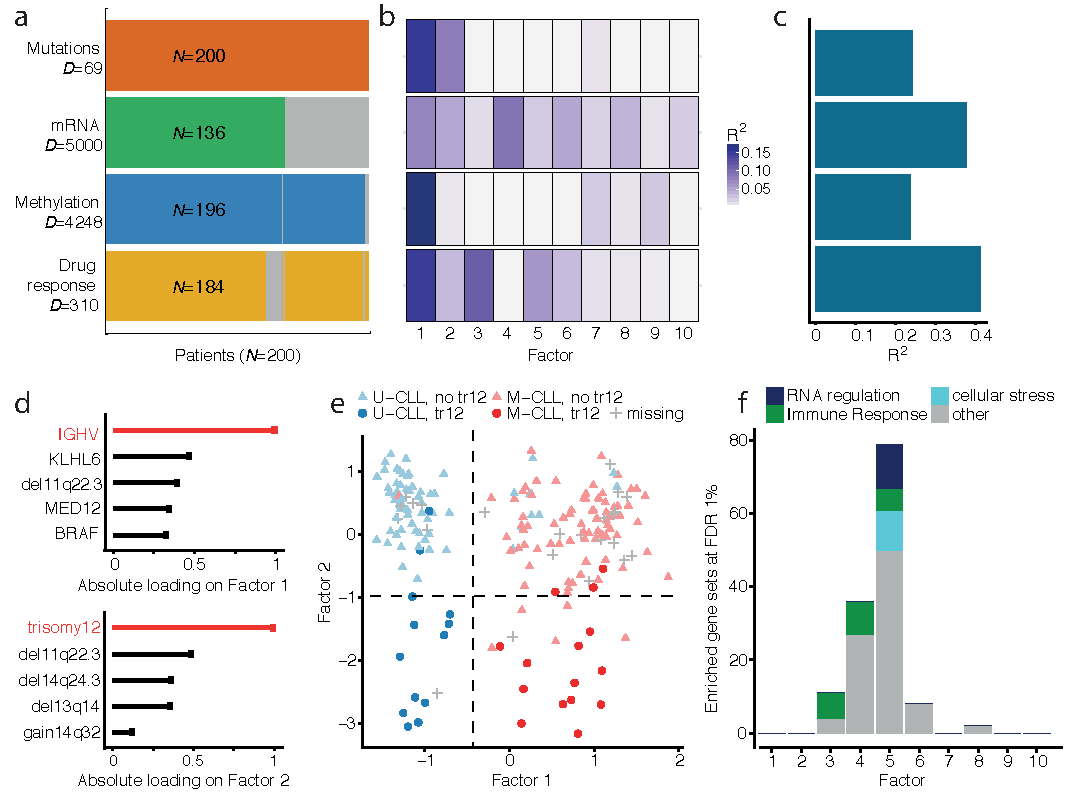
\includegraphics[width=1.0\textwidth]{MOFA_CLL_Figure1}
	\caption{XX}
	\label{fig:MOFA_CLL_Figure1}
\end{figure}

\subsubsection{Characterisation of Factor 1}

IGHV status is probably the most important prognostic marker in CLL and has routinely been used to distinguish between two distinct subtypes of the disease. Molecularly, it is a surrogate of the level of activation of the B-cell receptor, which is in turn related to the differentiation state of the tumoral cells. Multiple studies have associated mutated IGHV with a better resposne to chemoimmunotherapy, whereas unmutated IGHV patients have a worse prognosis \cite{Fabbri2016,Bulian2017,Crombie2017,Damle1999}.\\

In clinical practice, the IGHV status has been generally considered binary. However, our results suggest a more complex structure with at least three groups or a potential underlying continuum, as also suggested in \cite{Oakes2016,Queiros2015}.\\
Interestingly, there is some discrepancy between the IGHV status predicted by MOFA and the IGHV status reported in the clinical data. Out the 200 patients, MOFA classifies 176 in accordance with the clinical label, it classifies 12 patients that lacked the clinical marker and it re-classifies 12 patients to the opposite group.\\
To validate the MOFA-based classification, we inspected the molecular profiles. sample-to-sample correlation matrices for the individual layers suggest that for 3 of the cases where the inferred factor disagrees with the clinical label, the molecular data supports the predicted label. The other 9 cases showed intermediate molecular sgnatures now well captured by the binary classification.\\
%Based on these results, we hypothesize that a multi-omics approach based on several molecular signatures could be a more precise and robust approach to predict clinical phenotypes than the use of single features such as mutations or expression of marker genes.

\begin{figure}[H]
	\centering 	
	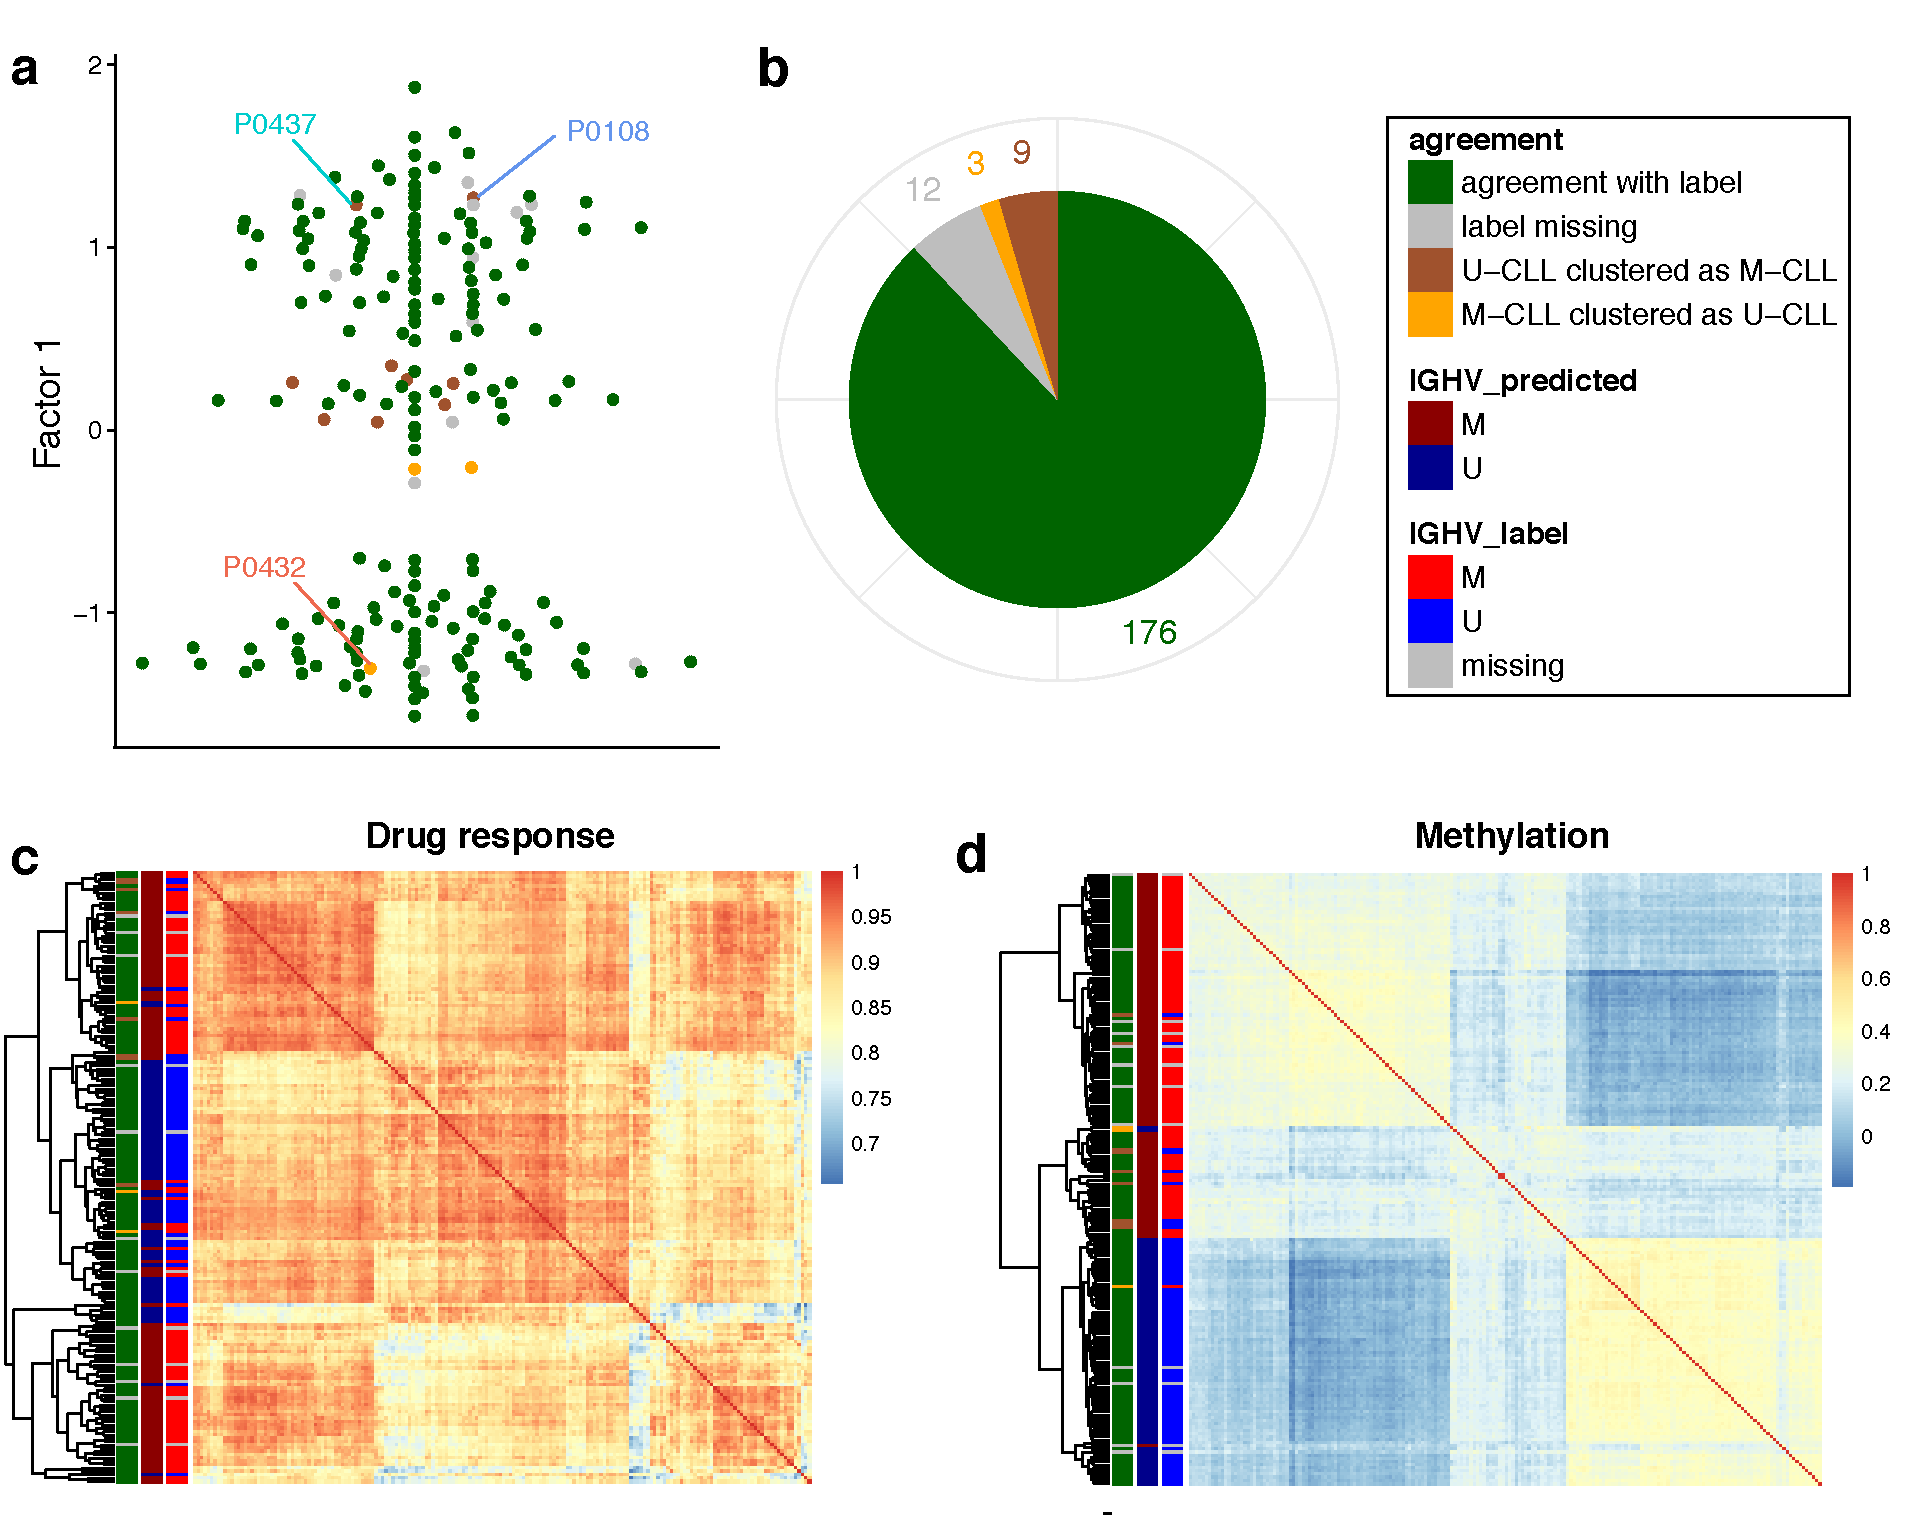
\includegraphics[width=1.0\textwidth]{MOFA_IGHV_outlier}
	\caption{XX}
	\label{fig:MOFA_IGHV_outlier}
\end{figure}


Finally, we characterised in more detail the molecular changes associated with IGHV status, as predicted by MOFA.\\
On the RNA expression, inspection of the top weights pinpoint genes that have been previously associated to IGHV status, some of which have been proposed as clinical markers\cite{Vasconcelos2005,Maloum2009,Trojani2011,Morabito2015,Plesingerova2017}. Heatmaps of the RNA expression levels for these genes reveals clear differences between samples when ordered according to the corresponding Factor 1 values.\\
On the drug response data the loadings highlight kinase inhibitors targeting the B-cell receptor pathway. Splitting the patients into three groups based on k-means clustering shows clear separation in the drug response curves.

\begin{figure}[H]
	\centering 	
	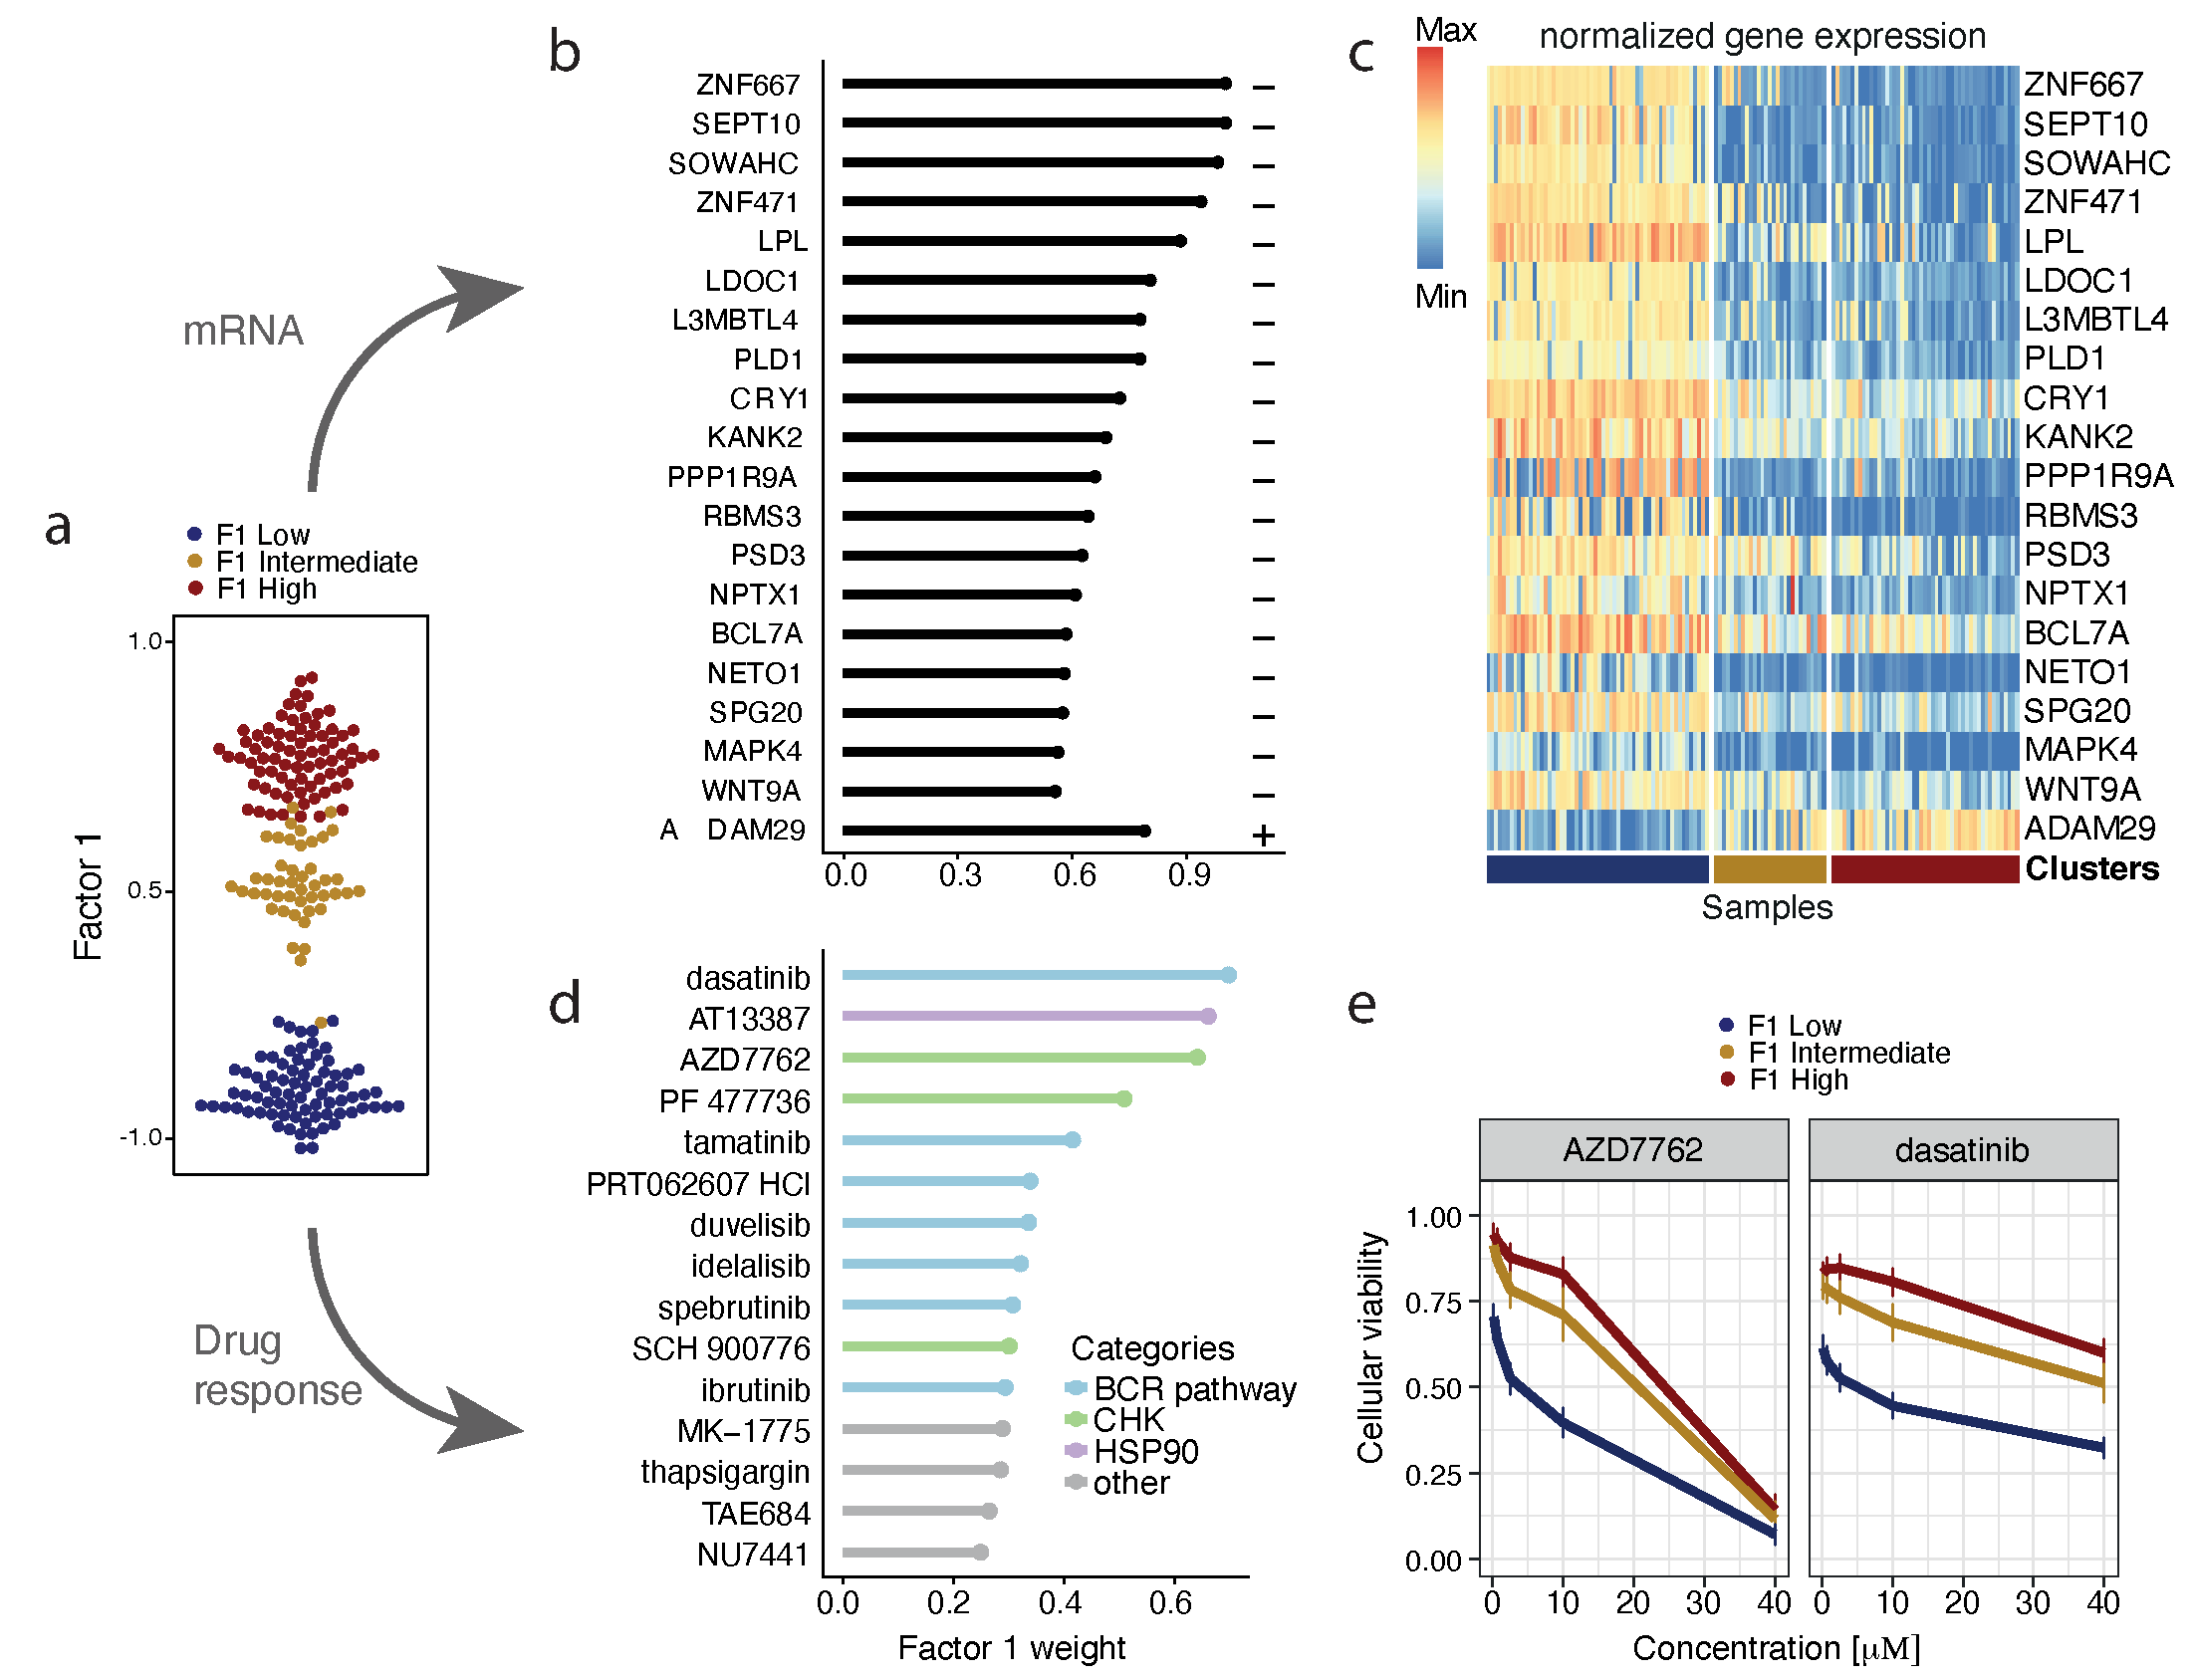
\includegraphics[width=1.0\textwidth]{MOFA_CLL_Factor1}
	\caption{XX}
	\label{fig:MOFA_CLL_Factor1}
\end{figure}

\subsubsection{Characterisation of other Factors}
% While the well-known clinical markers such as IGHV status and the more recently studied trisomy 12 are identified as most important sources of variation, they explain less than 20% variability in any view, suggesting the existence of more subtle sources of variation. 
% As an example, we further investigated latent factor 5, which explains 2% variation in the mRNA view and 6% of variation in the drug response view and is highly enriched for oxidative stress and senescence pathways in the mRNA view (Figure S12a). In particular, the top weights correspond to heat shock proteins (HSPs) such as HSPA1A, HSPA1B and HSPA6 (Figure S12b), a group of proteins that are essential for protein stability which are up-regulated upon stress conditions like high temperatures, pH shift or oxidative stress. Importantly, in tumour cells, including CLL, HSPs have been described to be elevated and may contribute to prolonged tumour cell survival (Dempsey et al. 2010a).
% In agreement with the findings from the mRNA view, the drugs with largest weights on factor 5 belong to clinical categories also associated with stress response, such as target reactive oxygen species (SD07, MIS-43, SD51) and DNA damage response (fludarabine, nutlin-3, doxorubicine) (Figure S12c-d). In particular, patients with high expression of HSPs display higher viability to the aforementioned drugs.

\subsubsection{Prediction of clinical outcomes}


We conjectured that the integration of the multiple molecular layers could allow a better prediction of clinical response compared to using single omics or naive data integration.\\
To evaluate the utility of the MOFA factors as predictors of clinical outcomes we fit Cox regression models \cite{Cox1972} using the patients' time to next treatment (TTT) as a response variable. Two types of analysis were performed: a univariate analysis where each Factor was independently associated with TTT, and a multivariate analysis where the combination of all Factors were used to predict TTT.\\

(CHECK) In the univariate Cox models, we observe  that Factor 1 (IGHV status), Factor 7 (associated with chemo-immunotherapy treatment prior to sample collection) and Factor 8 (Wnt signalling) were significant predictors of TTT. Accordingly, when splitting patients into binary groups based on the corresponding factor values, we observe clear differences in the survival curves.\\

In the multivariate Cox model, MOFA (Harrell's C-Index C=0.78) outperformed all other input settings, including single-omic data (C=0.68-0.72), individual genetic markers (C=0.66) as well the concatenated data matrix (C=0.74).

%As predictors, we included the top 10 principal components calculated on the data for each single view, a concatenated data set ('all') as well as the 10 MOFA factors. Missing values in a view were set to the feature-wise mean. In a second set of models, we used the complete set of all features in a view with a ridge penalty in the Cox model as imple- mented in the R package glmnet. For the Kaplan-Meier plots, an optimal cut-point on each factor was determined to define the two groups using the maximally selected rank statistics as implemented in the R package survminer with P-values based on a log-rank test between the resulting groups.

\begin{figure}[H]
	\centering 	
	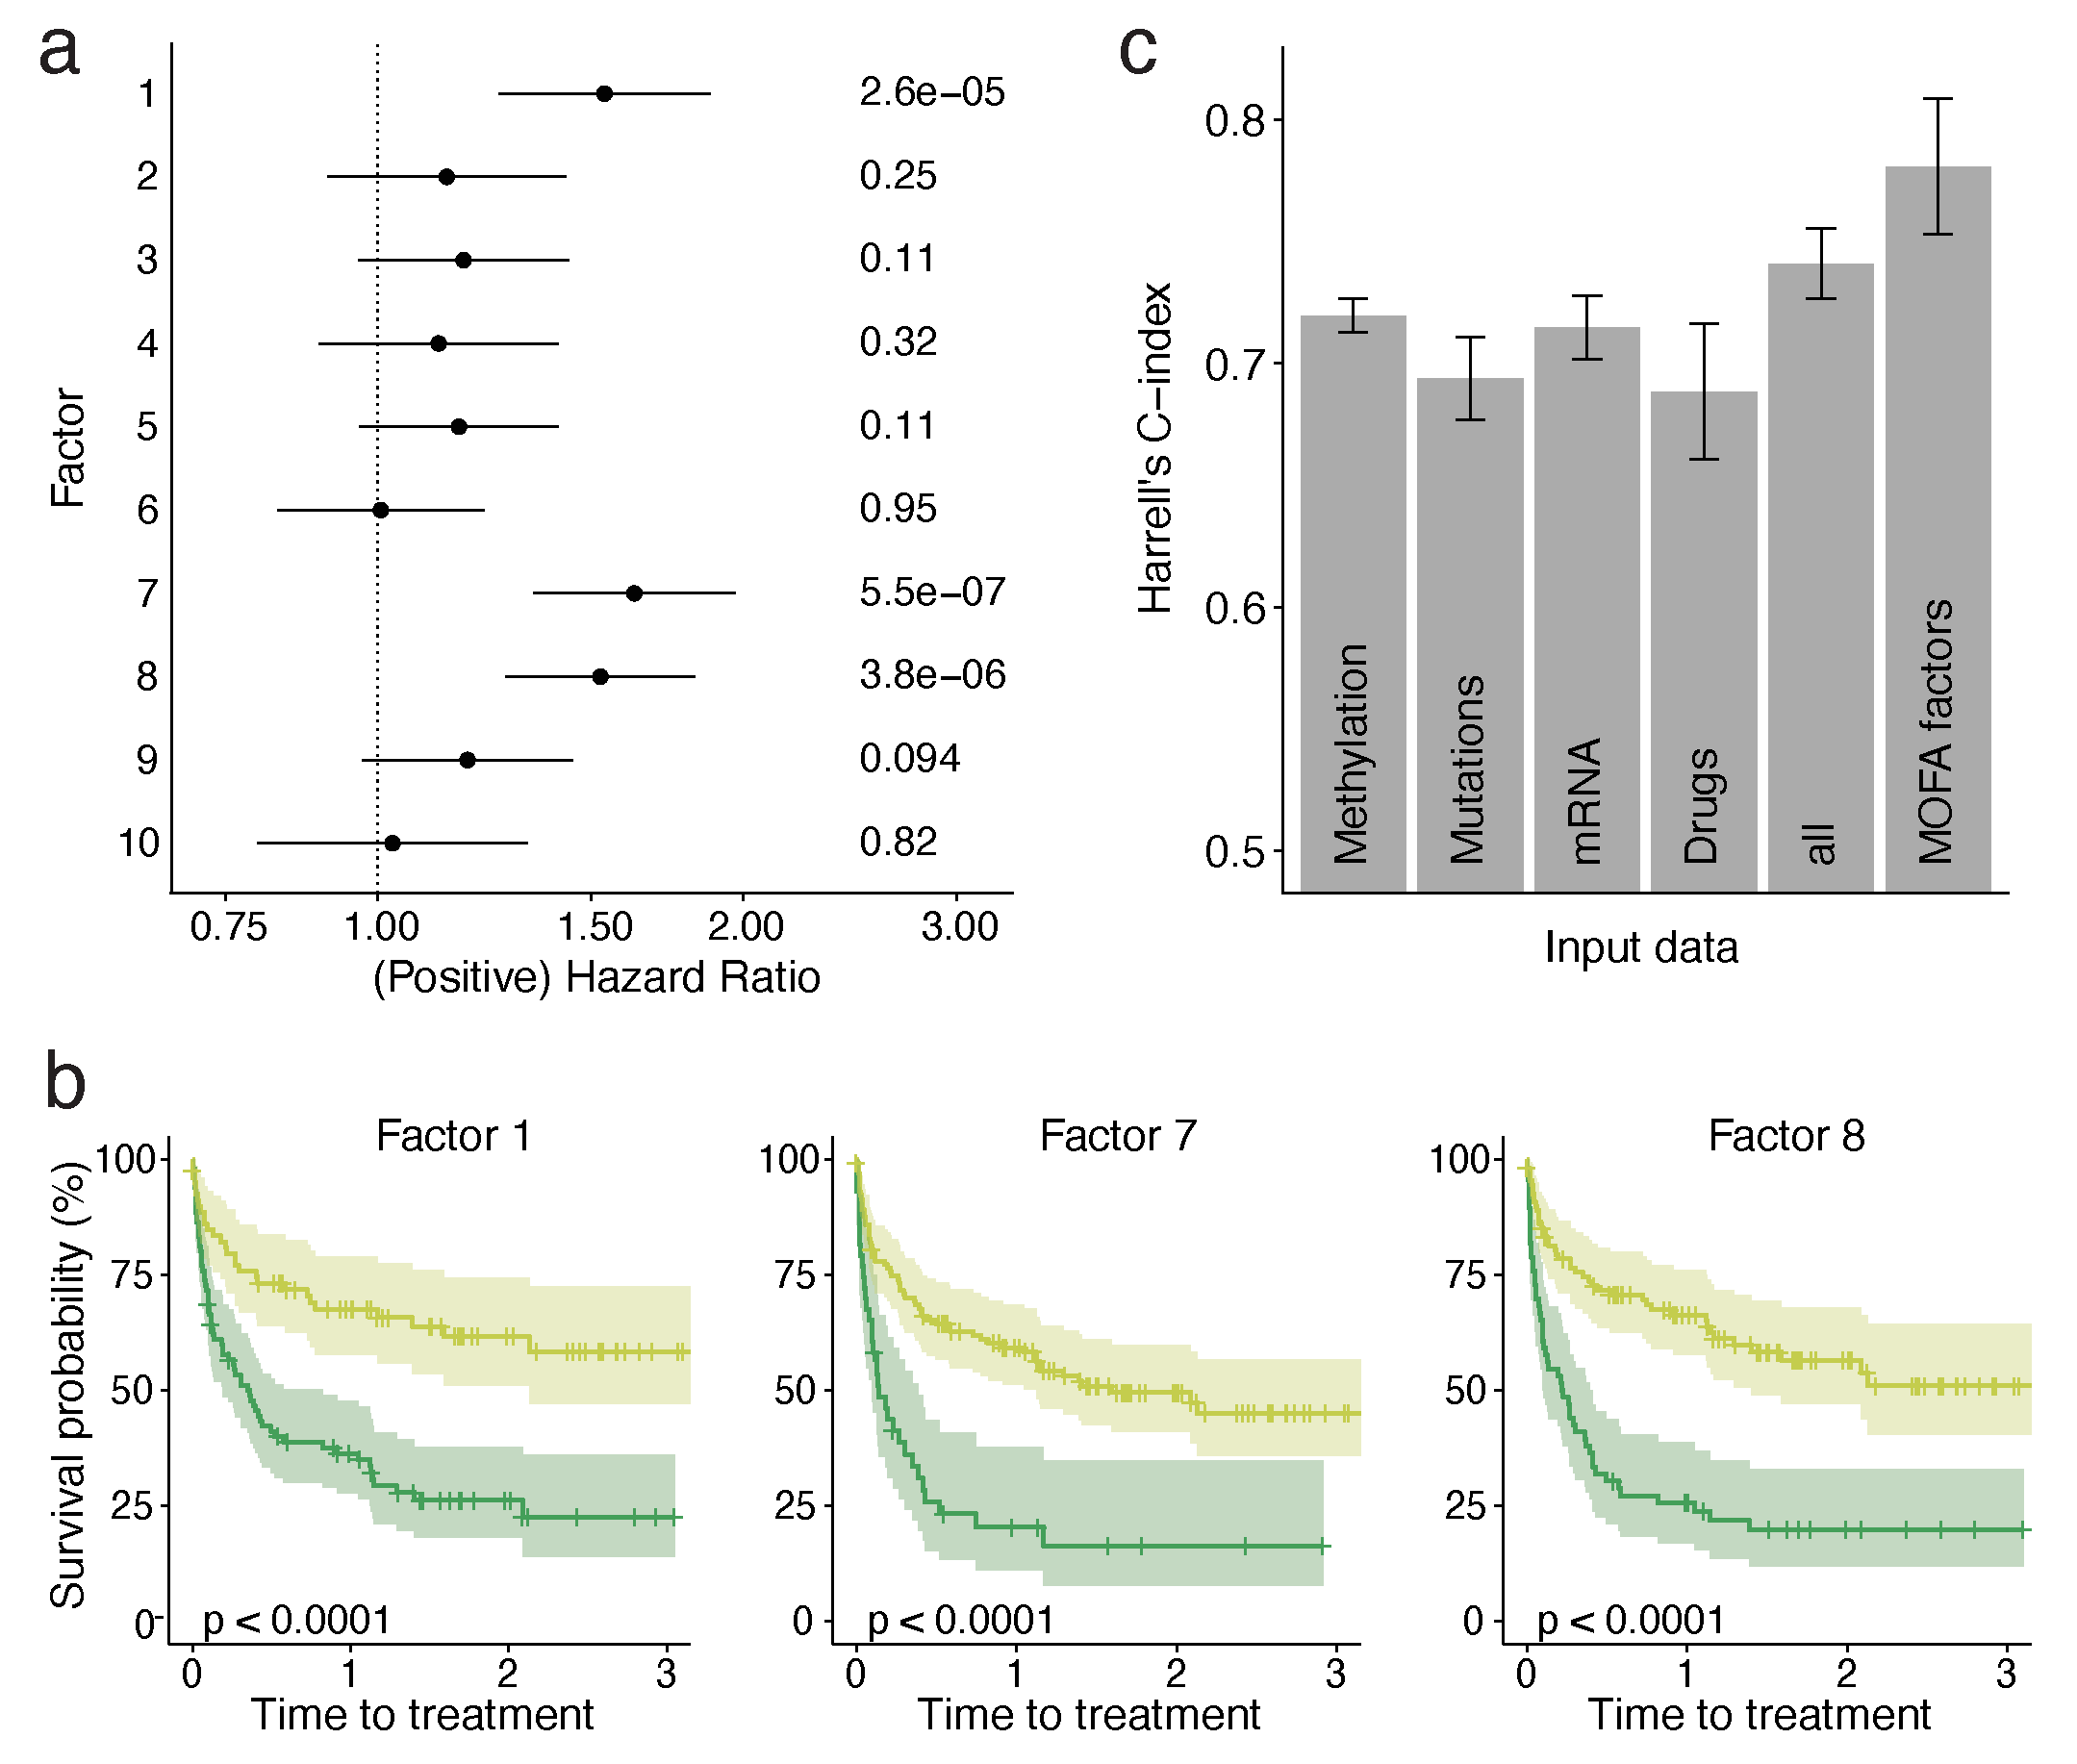
\includegraphics[width=0.9\textwidth]{MOFA_CLL_Cox}
	\caption{XX}
	\label{fig:MOFA_CLL_Cox}
\end{figure}


\subsubsection{Imputation of missing values}

A promising application of MOFA is the imputation of missing values as well as entire missing assays, which could massively reduce experimental costs.\\
The principle of imputation in MOFA follows the same logic as simulating from the generative model: if the factors and weights are available one can reconstruct the data by a simple matrix multiplication:
\[
	\hat{\bfY} = \E[\bfZ] \E[\bfW]^T
\]
where $\E[\bfZ]$ and $\E[\bfW]$ denote the expected values of the variational distributions for the factors and the loadings, respectively. Instead of point estimates, more advanced and fully Bayesian posterior predictive distribution could be obtained by propagating the uncertainity \cite{Gelman2013}. Yet, given that the variance of the variational distributions tend to be heavily underestimated (see \Cref{section:expectation_propagation}), we did not attempt this approach.\\

To assess the imputation performance, we trained MOFA models on patients with complete measurements after masking parts of the drug response data. In a first experiment, we masked values at random, and in a second experiment we masked the entire drug response data. 
We compared the results to some established imputation strategies, including imputation by feature-wise mean, SoftImpute \cite{Mazumder2010}, a k-nearest neighbour method \cite{Troyanskaya2001}.\\

For both imputation tasks, MOFA consistently yielded more accurate predictions, albeit the differences became less pronounced in the imputation of full assays, a more challenging task.

\begin{figure}[H]
	\centering 	
	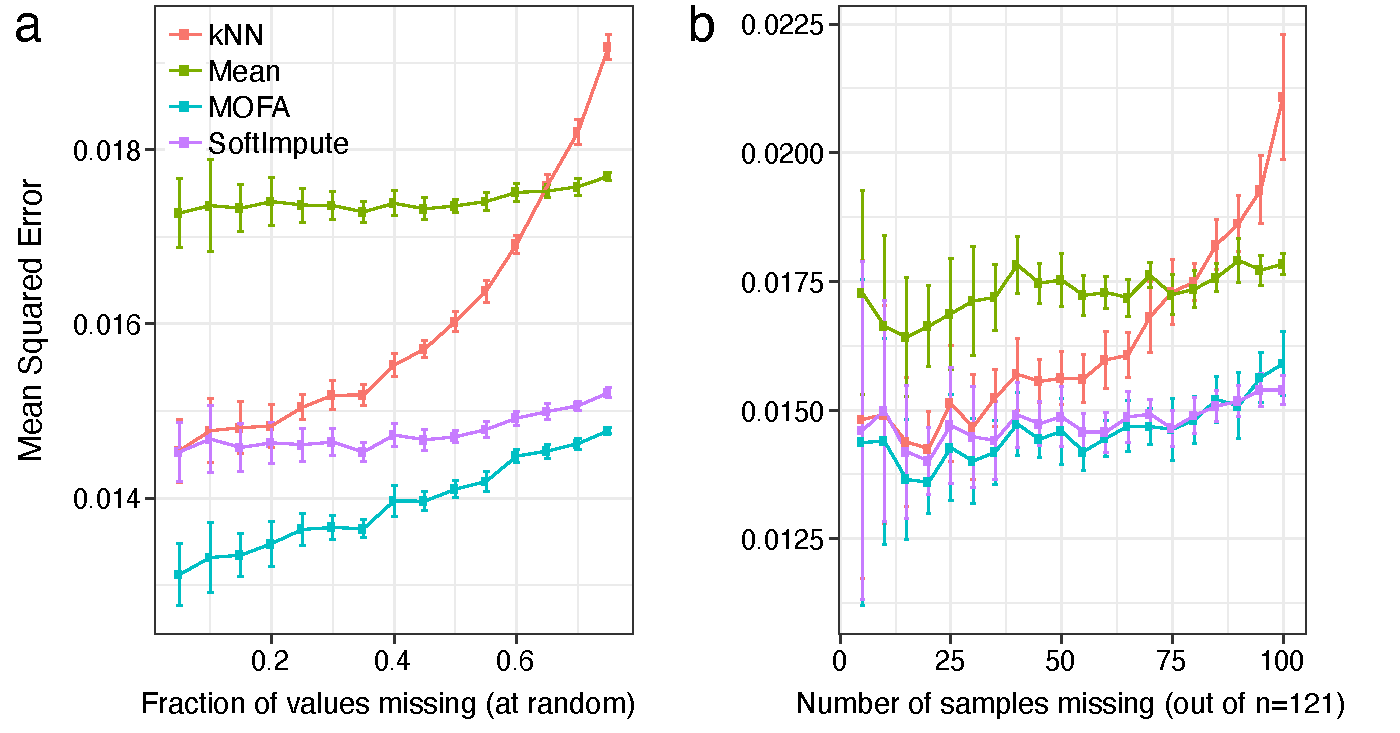
\includegraphics[width=1.0\textwidth]{MOFA_imputation}
	\caption{Evaluation of imputation performance in the drug response assay of the CLL data. The y-axis shows averages of the mean-squared error across 15 trials for increasing fractions of missing data (x-axis). Two experiments were considered: (a) values missing at random and (b) entire assays missing at random. Error bars represent standard deviations.}
	\label{fig:MOFA_imputation}
\end{figure}

% TO-DO: ADD EXAMPLES


\subsection{Application to single-cell multi-omics} \label{section:mofa_scmt}
The emergence of single-cell multi-modal techniques has created open opportunities for the development of novel computational techniques that integrate data sets across multiple modalities \cite{Stuart2019,Colome-Tatche2018,Chappell2018}. Here, we investigated the potential of MOFA to unravel the heterogeneity in one of the earliest single-cell multi-omics experiments \cite{Angermueller2016}.\\
The data set consists on 87 embryonic stem cells (ESCs) where RNA expression and DNA methylation were simultaneously measured using single-cell Methylation and Transcriptome sequencing (scM\&T-seq). Two populations of ESCs were profiled: the first one contains 16 cells grown in 2i media, which induces a native pluripotency state with genome-wide DNA hypomethylation \cite{Ficz2013}. the second population contains 71 cells grown in serum media, which triggers a primed pluripotency state poised for differentiation \cite{Tosolini2016}.\\

The RNA expression data was processed using standard pipelines to obtain log normalised counts, followed by a selection of the top 5,000 most overdispersed genes \cite{Lun2016}.\\
The DNA methylation data was processed as described in Chapter 1. Briefly, for each CpG site, we calculated a binary methylation rate from the ratio of methylated read counts to total read counts. Next, CpG sites were classified by overlapping with genomic contexts, namely promoters, CpG islands and enhancers (defined by the presence of distal H3K27ac marks). Finally, for each annotation we selected the top 5,000 most variable CpG sites with a minimum coverage of 10\% across cells.\\
Each of the resulting matrices was defined as a separate view for MOFA. The methylation data was modelled with a Bernoulli likelihood and the RNA expression data was modelled with a Gaussian likelihood.\\

In this data set, MOFA learnt 3 factors (minimum explained variance of 1\%). Factor 1 captured the transition from naive to primed pluripotent states, which MOFA links to widespread coordinated changes between DNA methylation and RNA expression (\Cref{fig:MOFA_scMT,fig:MOFA_scMT2}. Inspection of the gene loadings for Factor 1 pinpoints important pluripotency markers including  Rex1/Zpf42 or Essrb \cite{Mohammed2017}. As previously described both in vitro \cite{Angermueller2016}) and in vivo \cite{Auclair2014}, the dynamics of DNA methylation are driven by a genome-wide increase in DNA methylation levels.\\
Factor 2 captured a second dimension of heterogeneity driven by the transition from a primed pluripotency state to a differentiated state, with RNA loadings enriched with canonical differentiation markers including keratins and annexins \cite{Fuchs1988}.\\

Jointly, the combination of Factors 1 and 2 reconstruct the coordinated changes between the transcriptome and the epigenome along the differentiation trajectory from naive pluripotent cells to differentiated cells. When applying popular integrative clustering algorithms \cite{Wang2014,Shen2009,Mo2013}, the trajectory is not recovered \Cref{fig:MOFA_scMT_clustering}, illustrating the importance of learning continuous latent spaces before applying clustering methods.

\begin{figure}[H]
	\centering 	
	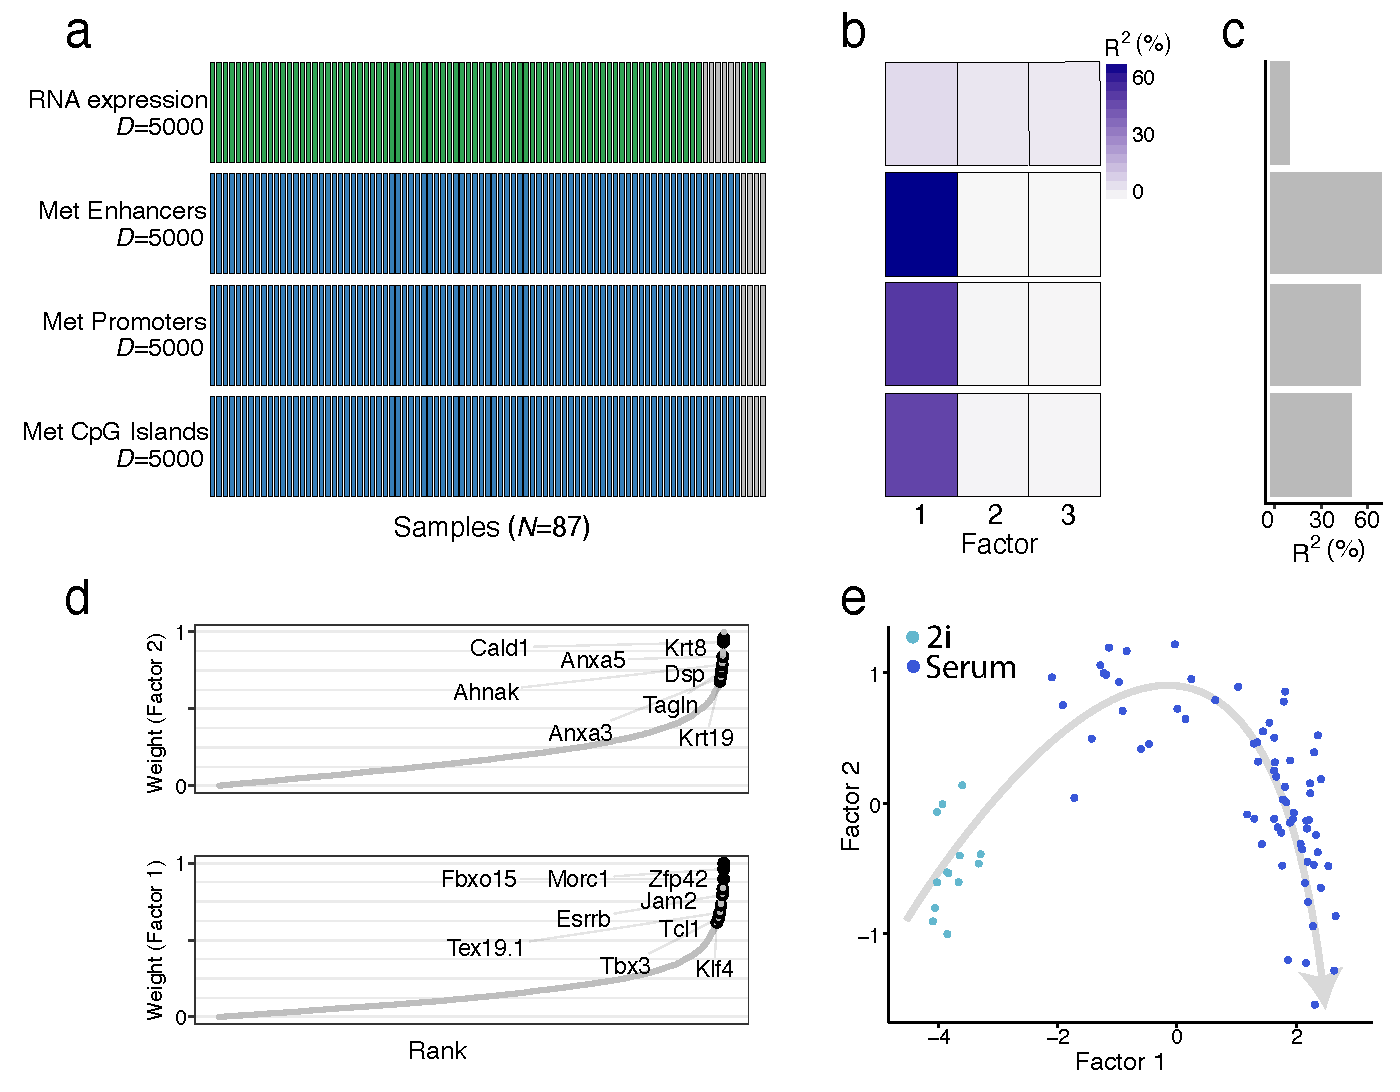
\includegraphics[width=1.0\textwidth]{MOFA_scMT}
	\caption{XX}
	\label{fig:MOFA_scMT}
\end{figure}

\begin{figure}[H]
	\centering 	
	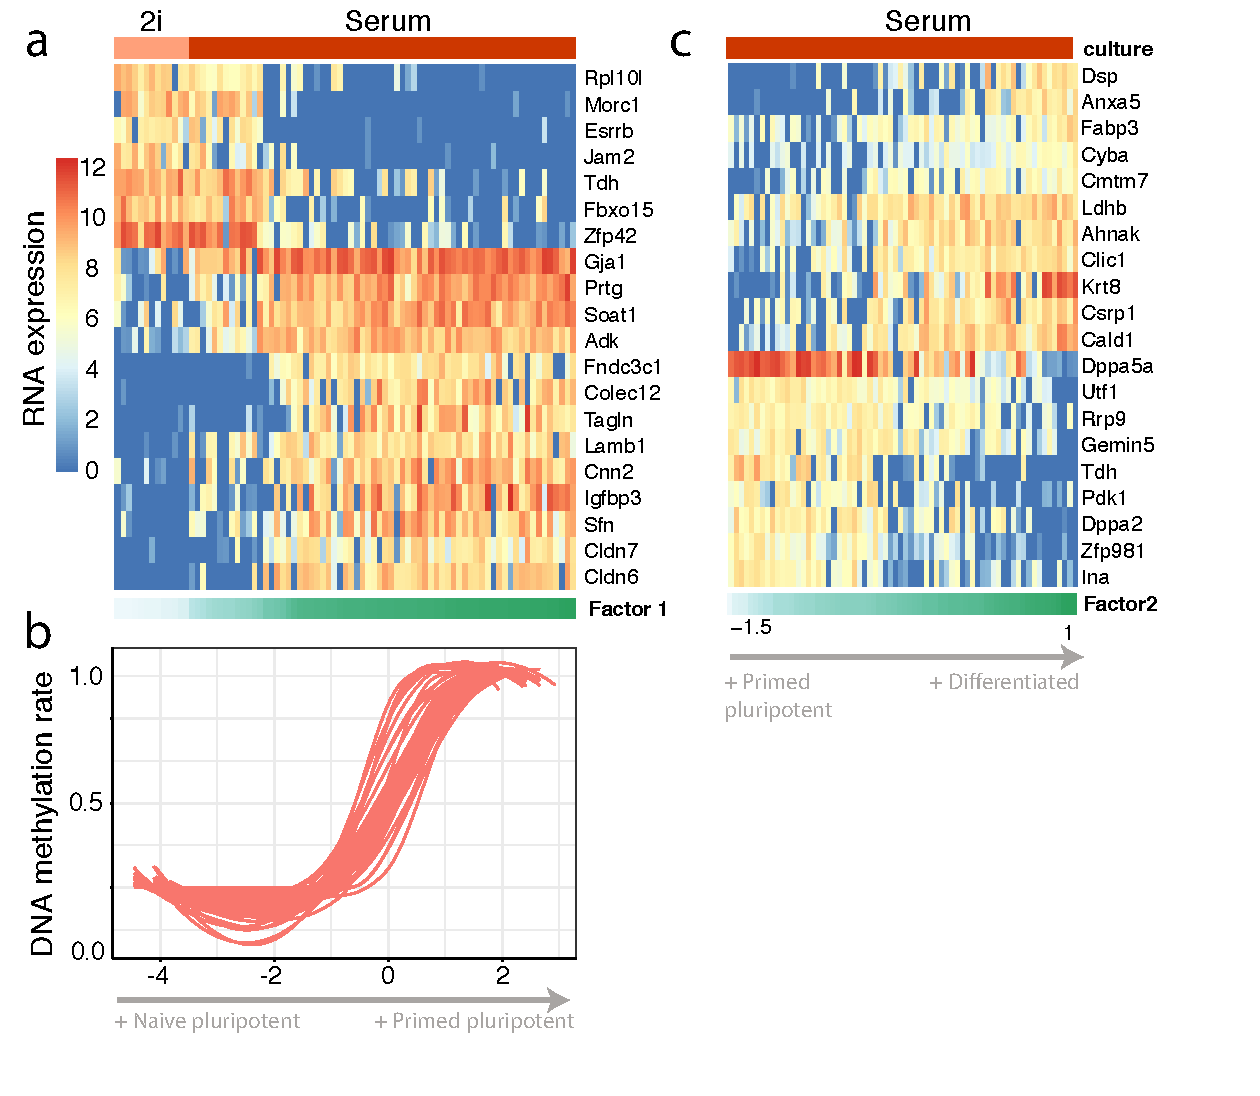
\includegraphics[width=1.0\textwidth]{MOFA_scMT2}
	\caption{XX}
	\label{fig:MOFA_scMT2}
\end{figure}

\begin{figure}[H]
	\centering 	
	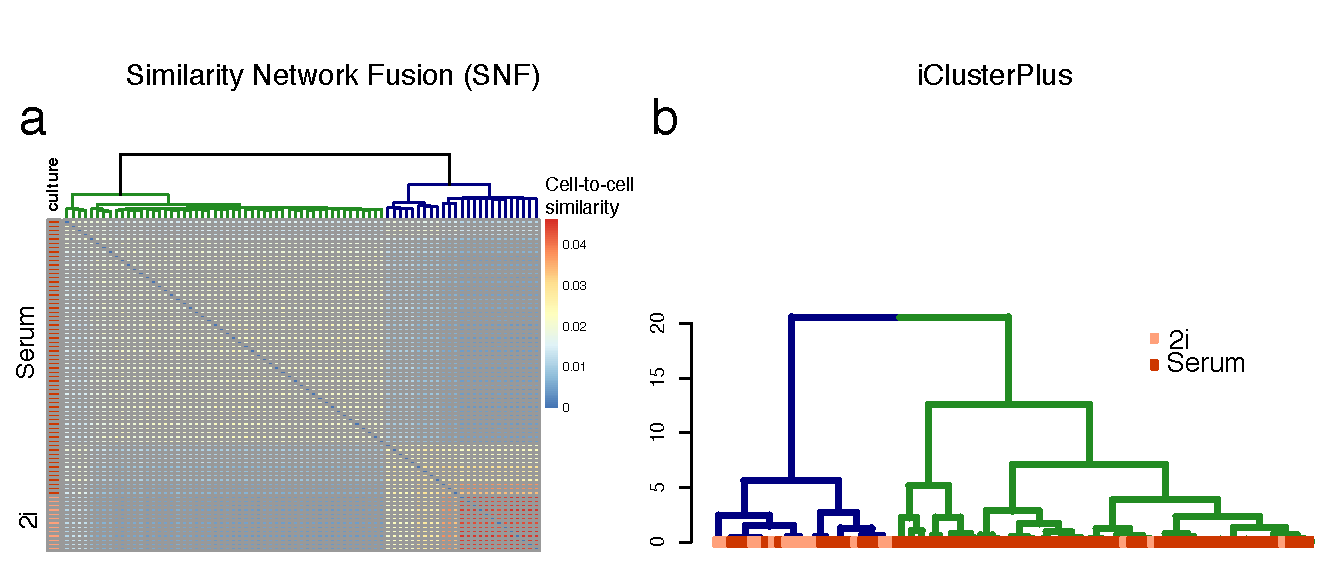
\includegraphics[width=1.0\textwidth]{MOFA_scMT_clustering}
	\caption{XX}
	\label{fig:MOFA_scMT_clustering}
\end{figure}


\subsection{Open perspectives}

MOFA addresses important challenges for the integrative analysis of multi-omics applications. Yet, the model is not free of limitations and there are open possibilities for future research, some of which we followed in Chapter 4.\\
\begin{itemize}

	\item \textbf{Linearity}: this is an assumption that is critical for obtaining interpretable feature loadings. Yet, as in any machine learning technique, there is often a trade-off between explanatory power and interpretability\cite{Kuhn}. Non-linear appproaches are particularly appealing in biology, where the drivers of variation often result from the complex (non-linear) interaction between potentially simple (and linear) processes. As such, non-linear approaches, including deep neural networks or variational autoencoders have shown promising results when it comes to dimensionality reduction \cite{Lin2017,Ding2018,Lopez2018}, batch correction\cite{Lopez2018}, denoising \cite{Eraslan2019} or imputation \cite{Lin2016}. Notably, few non-linear multi-view factor analysis models exist \cite{Damianou2016}, making it an interesting line of research.

	\item \textbf{Scalability}: the size of biological datasets is rapidly increasing, particularly in the field of single cell sequencing, with some studies reporting more than a milion cells\cite{Svensson2018,Cao2019}. \\
	When comparing to previous methods that make use of maximum likelihood or sampling-based Bayesian methods, the variatonal framework implemented in MOFA yields a notable improvement in scalability. Yet, in its vanilla form, variational inference becomes prohibitively slow with very large datasets \cite{Hoffman2013,Blei2016,Hoffman2014}, hence motivating the development of even more efficient inference schemes that potentially scale to milions of samples. This line of research is followed in Chapter 4, with the development of a stochastic version of the variational inference algorithm.

	\item \textbf{Sample independence assumption and generalisations to multi-group structures}: the sparsity assumptions in MOFA are based on the principle that features are structured into well-defined views. As such, the activity of the infered factors is also expected to be structured, so that different factors explain variability in different subsets of views (\Cref{fig:MOFA}). Following the same logic, many studies contain structured samples, as either multiple experiments or conditions. The integration of multiple sample groups requires breaking the assumption of independent samples and introducing a prior that captures the structured sparsity at the sample level. This line of research is followed in Chapter 4, with the introduction of a symmetric multi-group and multi-view sparsity prior.

	\item \textbf{Tailored likelihoods for single-cell analysis}: MOFA enables the modular extension to arbitrary non-gaussian likelihoods, provided that they can be locally bounded and integrated into the variational framework (see \Cref{section:mofa_ngaussian}). New likelihood models such as zero-inflated negative binomial distributions \cite{Risso2018} could make MOFA more suited to the analysis of single-cell data.

	\item \textbf{Bayesian treatment of predictions}: in the current implementation, after inference we extract point estimates for each variable, namely expectations. While convienient for plotting, this ignores the uncertainity associated with the estimates, one of the main strength of Bayesian methods. Future extensions could attempt a more comprehensive Bayesian treatment that propagates uncertainity in the downstream analyses, mainly when it comes to making predictions and imputation \cite{Gelman2013}.

	\item \textbf{Incorporation of prior information}: an unsupevised approach is appealing for discovering the principal axes of variation, but sometimes this can yield challenges in the interpretation of factors. Future extensions could exploit the rich information encoded in pathway databases, similar to the approach proposed in \cite{Buettner2017}.

\end{itemize}


